\documentclass[conference]{IEEEtran}
\IEEEoverridecommandlockouts
\usepackage{cite}
\usepackage{amsmath,amssymb}
\usepackage{algorithm}
\usepackage{algorithmic}
\usepackage{graphicx}
\usepackage{booktabs}
\usepackage{multirow}
\usepackage{textcomp}
\usepackage{url}

\begin{document}

\title{Deadline-Aware Elastic Provisioning for\\Hibernation-Tolerant Bag-of-Tasks Scheduling\\on Spot and Burstable Cloud Instances}

\author{\IEEEauthorblockN{}\IEEEauthorblockA{}}

\maketitle

\begin{abstract}
Spot virtual machines cut cloud compute prices substantially but may be
hibernated by the provider at any time, which threatens deadline-constrained
workloads. Burst-HADS tolerates such interruptions by migrating the tasks of a
hibernated instance onto burstable VMs running in burst mode, falling back to
on-demand capacity when no burstable instance is free. Because a burstable
instance accepts only one task at a time and the number provisioned is a fixed
fraction of the selected fleet, the rescue capacity available at the moment of
an interruption is bounded independently of how much work is actually
displaced. We present R-BurstHADS, which extends Burst-HADS's dynamic scheduler
with elastic spot provisioning drawn from the same instance catalogue, sized by
a work-conservation argument against the remaining deadline rather than by a
fixed queue-length constant. Across 7{,}200 runs per launch-limit setting (five
hibernation scenarios, four workload sizes, four deadline factors, 30 seeds,
three schedulers), R-BurstHADS shortens makespan in every configuration and
every regime we measured: 27.7\% below HADS and 12.0\% below Burst-HADS on the
full sweep, and 11.0\% below an unmodified Burst-HADS in the one regime where
that baseline needs no repair from us. That speed costs 2.9\% more money, and
the penalty is concentrated in small bags: 12.7\% dearer at 50 tasks and 9.6\%
at 100, in the same direction at every deadline factor and both launch-limit
settings we measured, and on the smallest bag it is no faster either. On the broader sweep, against our
own Burst-HADS, it is 4.6\% cheaper and dominates in 49 of 75 cells, but that
baseline carries three departures from the published algorithm which we
disclose and quantify, so we report a controlled comparison with a documented
fidelity audit rather than a reproduction.
\end{abstract}

\begin{IEEEkeywords}
cloud computing, spot instances, burstable instances, task scheduling,
hibernation, bag-of-tasks, deadline constraints
\end{IEEEkeywords}

\section{Introduction}

Infrastructure-as-a-Service providers sell surplus capacity at a steep discount
under names such as Amazon EC2 Spot~\cite{aws}. The discount is paid for in reliability:
the provider may reclaim the instance at short notice. Amazon EC2 additionally
offers \emph{hibernation}, in which the instance's memory and context are
written to its EBS root volume and execution is suspended rather than
destroyed, with the instance resuming when capacity becomes available again.
For a workload with a deadline, hibernation is not free even though the
checkpoint preserves progress: the capacity disappears for an unknown period,
and the displaced work must be placed somewhere else in time to finish.

Bag-of-Tasks (BoT) applications --- parameter sweeps, Monte Carlo simulation,
chromosome mapping, image processing --- are a natural fit for this market.
Their tasks are independent, so a lost instance costs only the work resident on
it, and the remaining tasks can in principle be redistributed freely.

Teylo et al. addressed this setting in two stages. HADS~\cite{hads2021}
schedules a BoT application across spot and non-burstable on-demand instances
and, when a spot VM hibernates, migrates its unfinished tasks to other running
instances or to newly launched on-demand ones. Burst-HADS~\cite{bursthads}
extends this with \emph{burstable} instances~\cite{t3}, which accumulate CPU credits
while idle and can then be driven at full processing power in burst mode; a
hibernation is answered first by migrating a task to an idle burstable VM,
and only then by falling back to on-demand capacity.

The rescue capacity Burst-HADS can call on at the instant of an interruption
is, however, fixed in advance. Its burstable fleet is sized once, after the
primary scheduling step, as a fixed fraction of the instances the search
selected, and a burstable instance holds only one task at a time so that
credits continue to accrue. Neither quantity depends on how much work a
hibernation actually displaces or on how much deadline slack remains when it
occurs. When the displaced work exceeds the standing burstable capacity, every
remaining task falls through to on-demand instances, which are the most
expensive resource in the catalogue and carry a start-up latency.

This paper makes the following contributions.

\begin{itemize}
\item We present \textbf{R-BurstHADS}, which adds two provisioning behaviours to
Burst-HADS: a risk-triggered \emph{preemptive} step (Algorithm~\ref{alg:preempt})
that launches a replacement spot instance for a high-risk VM before it is
interrupted, and a \emph{deadline-aware reactive} step
(Algorithm~\ref{alg:sizing}) that provisions the minimum additional capacity
required for the displaced work to finish before the deadline. Both draw from
the same instance catalogue available to the baselines.
\item We \textbf{audit the fidelity} of our baseline re-implementations against
the published results and disclose where they do not reproduce them, including
three measured departures of our Burst-HADS from the published algorithm
(Section~\ref{sec:validation}).
\item We evaluate all three schedulers under the \textbf{hibernation scenarios of
the source work} across four workload sizes, four deadline factors and 30
seeds, and separate what holds from what does not: the makespan advantage
holds in every configuration and regime measured, while against an unmodified
baseline the method is \textbf{consistently more expensive on small bags},
a negative result about our own scheduler that we report as ours
(Section~\ref{sec:results}).
\end{itemize}

\section{Background and Related Work}

\subsection{Scheduling on interruptible instances}

Work on interruptible cloud instances divides broadly into bidding and
checkpointing strategies for surviving reclamation, and scheduling strategies
that treat interruption as a first-class constraint. AutoBoT-like approaches
select instance types under a deadline and budget but do not model hibernation.
The line we build on schedules explicitly against a hibernation process.

\subsection{HADS and Burst-HADS}

HADS~\cite{hads2021}, developed from an earlier conference version~\cite{hadsconf},
formulates BoT scheduling on spot and on-demand instances
as a cost-minimisation problem under a deadline $D$, building a static map with
a greedy single-pass construction and migrating tasks away from hibernated
instances at runtime. Burst-HADS~\cite{bursthads} replaces the greedy
construction with an Iterated Local Search (ILS), adds burstable instances as a
rescue tier, and introduces a work-stealing procedure that rebalances load
whenever an instance becomes idle.

Because Burst-HADS's Burst Migration Procedure draws burstable candidates from
the idle set and moves each recipient to the busy set on assignment, a burstable
instance accepts exactly one migrated task at a time. Combined with a fleet size
fixed at scheduling time, this bounds the burstable rescue capacity independently
of the size of the interruption --- the gap this work addresses.

\section{System Model and Problem Formulation}

An application is a set $T$ of $|T|$ independent tasks with a common deadline
$D$. A task $t_i$ has execution time $e_i$ on a reference core and memory
requirement $m_i$. The provider offers a catalogue $M$ of VM types; $vm_j$ has
processing speed $s_j$, virtual core count $\mathit{nvc}_j$, memory $M_j$ and
price $c_j$ per unit time. A multi-core instance executes up to $\mathit{nvc}_j$
tasks simultaneously, one per core, so its whole-instance throughput is
$s_j\cdot \mathit{nvc}_j$. Symbols are collected in Table~\ref{tab:vars}.

\begin{table}[t]
\caption{Variables and parameters used in the algorithms}
\label{tab:vars}
\centering
\footnotesize
\begin{tabular}{ll}
\toprule
Symbol & Meaning \\
\midrule
$T$, $t_i$ & task set; task $i$ \\
$e_i$, $m_i$ & execution time and memory requirement of $t_i$ \\
$e_{ij}$ & execution time of $t_i$ on $vm_j$ \\
$M$, $vm_j$ & VM catalogue; instance $j$ \\
$s_j$, $\mathit{nvc}_j$ & speed and virtual-core count of $vm_j$ \\
$M_j$, $c_j$ & memory capacity and price per period of $vm_j$ \\
$\Theta(\cdot)$ & throughput of a VM set, $\sum_j s_j\!\cdot\!\mathit{nvc}_j$ \\
$D$ & application deadline \\
$D_{\mathit{spot}}$ & deadline minus the worst-case migration reserve \\
$\mathit{RD}_{\mathit{spot}}$ & relaxed $D_{\mathit{spot}}$ used inside the ILS \\
$\omega$ & checkpoint overhead fraction \\
$T_{\mathit{start}}$ & instance start-up latency \\
$\mathit{cc}_j$, $\mathit{rcc}_{ij}$ & accrued and required CPU credits \\
$\lambda_h$, $\lambda_r$ & hibernation and resumption rates \\
$k_h$, $k_r$ & expected hibernations / resumptions over $D$ \\
$S$, $S_{\mathit{best}}$ & candidate and incumbent scheduling solutions \\
$\alpha$ & cost/makespan weight in the fitness function \\
$\mathit{burst\_rate}$ & burstable fleet size as a fraction of $|S|$ \\
$Q_l$ & unfinished tasks of a hibernated instance $vm_l$ \\
$\mathit{IR}$, $\mathit{BR}$ & sets of idle and busy instances \\
$M^{o}$, $M^{b}$ & elastic on-demand and burstable pools \\
$A$ & active replacement instances provisioned at runtime \\
$W$ & remaining work of the tasks awaiting placement \\
$\rho$ & preemptive provisioning risk threshold \\
$p_v$ & hibernation probability of $vm_v$ over one task \\
\bottomrule
\end{tabular}
\end{table}

Cost is instance-seconds: an instance is charged from launch until termination
or hibernation, whether or not it is executing. The objective is
\begin{equation}
\min\ \alpha \cdot \widehat{\mathit{cost}} + (1-\alpha)\cdot \widehat{\mathit{mkp}}
\quad \text{s.t.}\quad \mathit{mkp} \leq D
\label{eq:fitness}
\end{equation}
over normalised cost and makespan. Candidate instances are ranked by
\begin{equation}
\mathit{weight}(vm_j) = \frac{\mathit{Gflops}_j}{c_j} = \frac{s_j \cdot \mathit{nvc}_j}{c_j}
\label{eq:wrr}
\end{equation}
where $\mathit{Gflops}_j$ quantifies the whole instance's computing power.
Placement on spot instances is constrained not by $D$ but by
\begin{equation}
D_{\mathit{spot}} = D - \max_i \frac{e_i \cdot (1+\omega)}{s_{\min}}
\label{eq:dspot}
\end{equation}
a reserve guaranteeing that the longest task can still be migrated to the
slowest instance and executed before $D$ if its host hibernates.

\section{R-BurstHADS}
\label{sec:design}

R-BurstHADS inherits Burst-HADS's ILS (Algorithm~\ref{alg:primary}), greedy
construction (Algorithm~\ref{alg:greedy}), local search
(Algorithm~\ref{alg:ls}), burst migration (Algorithm~\ref{alg:migrate}) and
work stealing (Algorithm~\ref{alg:steal}), and adds two provisioning
behaviours, Algorithms~\ref{alg:preempt} and~\ref{alg:sizing}. Both launch spot
instances of the most cost-efficient spot type present in the scheduler's own
pool, $\arg\max_j s_j\mathit{nvc}_j/c_j$, so the proposed method has access to
no instance type the baselines cannot also select. The per-task tier falls back
to a burstable instance when a spot instance cannot be launched within the
account limits or would breach the spare-time margin of
Eq.~(\ref{eq:dspot})'s reserve. Every instance either behaviour launches, spot
or burstable, is usable only after $T_{\mathit{start}}$. Table~\ref{tab:algprov} lists the
provenance of every algorithm the scheduler executes; all seven are reproduced
here so that the method can be implemented from this paper alone.

\begin{table}[t]
\caption{Provenance of the algorithms R-BurstHADS executes}
\label{tab:algprov}
\centering
\footnotesize
\begin{tabular}{@{}llp{3.0cm}@{}}
\toprule
Alg. & Source & Role \\
\midrule
\ref{alg:primary} & Burst-HADS~\cite{bursthads} & iterated local search over the static schedule \\
\ref{alg:greedy}  & Burst-HADS~\cite{bursthads} & initial solution \\
\ref{alg:ls}      & Burst-HADS~\cite{bursthads} & neighbourhood search \\
\ref{alg:preempt} & \textbf{this work} & preemptive provisioning (Theorem 1) \\
\ref{alg:sizing}  & \textbf{this work} & deadline-aware sizing (Theorem 2) \\
\ref{alg:migrate} & Burst-HADS~\cite{bursthads} & burstable rescue on hibernation \\
\ref{alg:steal}   & Burst-HADS~\cite{bursthads} & work stealing on idle \\
\bottomrule
\end{tabular}
\end{table}

\begin{algorithm}[t]
\caption{Primary scheduler: iterated local search. Inherited from Burst-HADS~\cite{bursthads}; the guarded move marked in the listing is ours.}
\label{alg:primary}
\begin{algorithmic}[1]
\STATE $D_{\mathit{spot}} \leftarrow$ Eq.~(\ref{eq:dspot})
\STATE $S \leftarrow \textsc{GreedyInitial}(T, M, D_{\mathit{spot}})$
\STATE $S_{\mathit{best}} \leftarrow \textsc{LocalSearch}(S, D_{\mathit{spot}})$
\STATE $\mathit{RD}_{\mathit{spot}} \leftarrow D_{\mathit{spot}}$;\ \ $it_b \leftarrow 0$;\ \ $it_r \leftarrow 0$
\FOR{$it = 1$ to $\mathit{max\_iteration}$}
  \IF{unused spot instances remain}
    \STATE add one at random to $S.\mathit{selected}$
  \ENDIF
  \IF{$it - it_b > \mathit{max\_failed}$ \AND $it - it_r > \mathit{max\_failed}$}
    \STATE $\mathit{RD}_{\mathit{spot}} \leftarrow \min\!\big(\mathit{RD}_{\mathit{spot}}(1+\mathit{relaxed\_rate}),\, D\big)$
    \STATE $it_r \leftarrow it$
  \ENDIF
  \STATE $S' \leftarrow \textsc{LocalSearch}(S, \mathit{RD}_{\mathit{spot}})$
  \IF{$\mathit{fitness}(S') < \mathit{fitness}(S_{\mathit{best}})$} \COMMENT{Eq.~(\ref{eq:fitness})}
    \STATE $S_{\mathit{best}} \leftarrow S'$;\ \ $it_b \leftarrow it$
  \ENDIF
  \STATE $S \leftarrow S'$
\ENDFOR
\STATE $n_b \leftarrow \lceil \mathit{burst\_rate}\cdot|S_{\mathit{best}}.\mathit{selected}|\rceil$
\STATE $B \leftarrow \textsc{LaunchBurstable}(n_b)$ from $M^{b}$, each ready at $T_{\mathit{start}}$
\FORALL{$t_i$ with predicted finish $> D_{\mathit{spot}}$, latest first}
  \STATE $b \leftarrow$ next free instance of $B$;\ \ \textbf{if} $b = \varnothing$ \textbf{then break}
  \IF{baseline finish of $t_i$ on $b$ improves on its current finish}
    \STATE move $t_i$ to $b$ in baseline mode
  \ENDIF \COMMENT{the test is \emph{ours}, not~\cite{bursthads}; Sec.~\ref{sec:validation}}
\ENDFOR
\STATE \COMMENT{\cite{bursthads} \S3.2 here sends the violators still on spot to the cheapest regular on-demand instances. We do not implement that step; Sec.~\ref{sec:validation}}
\FORALL{instances $b \in B$ still free}
  \STATE $t_i \leftarrow$ latest-finishing task not already on $b$
  \IF{$b$ fits $t_i$ \AND baseline finish of $t_i$ on $b$ improves on its current finish}
    \STATE move $t_i$ to $b$ in baseline mode
  \ENDIF \COMMENT{same test of ours}
\ENDFOR
\STATE \textsc{PreemptiveProvision}($S_{\mathit{best}}$) \COMMENT{Alg.~\ref{alg:preempt}}
\RETURN $S_{\mathit{best}}$
\end{algorithmic}
\end{algorithm}

\begin{algorithm}[t]
\caption{\textsc{GreedyInitial}: initial solution. Inherited from Burst-HADS~\cite{bursthads}.}
\label{alg:greedy}
\begin{algorithmic}[1]
\STATE sort $T$ by memory requirement, descending
\FORALL{$t_i \in T$}
  \FORALL{$vm_j \in \mathit{selected}$, least loaded first}
    \IF{$\textsc{Feasible}(t_i, vm_j, D_{\mathit{spot}})$}
      \STATE assign $t_i$ to $vm_j$; \textbf{continue} with next task
    \ENDIF
  \ENDFOR
  \STATE $K \leftarrow \{vm_j \in M^{s}\setminus \mathit{selected} : \textsc{Feasible}(t_i,vm_j,D_{\mathit{spot}})\}$
  \STATE $vm_j \leftarrow \textsc{WrrPick}(K)$ using Eq.~(\ref{eq:wrr})
  \IF{$vm_j \neq \varnothing$}
    \STATE select and assign; \textbf{continue} with next task
  \ENDIF
  \FORALL{on-demand $vm_j$ with launch room, cheapest first}
    \IF{$\textsc{Feasible}(t_i, vm_j, D)$}
      \STATE assign; \textbf{continue} with next task
    \ENDIF
  \ENDFOR
  \STATE $vm_{\mathit{new}} \leftarrow \textsc{LaunchOnDemand}()$ from $M^{o}$
  \IF{$\textsc{Feasible}(t_i, vm_{\mathit{new}}, D)$}
    \STATE assign
  \ELSE
    \STATE \textbf{abort}: no feasible placement before $D$
  \ENDIF
\ENDFOR
\end{algorithmic}
\end{algorithm}

\begin{algorithm}[t]
\caption{\textsc{LocalSearch}. Inherited from Burst-HADS~\cite{bursthads}.}
\label{alg:ls}
\begin{algorithmic}[1]
\REQUIRE solution $S$, bound $d$
\STATE $\mathit{best} \leftarrow S$
\STATE $\mathit{dest} \leftarrow$ one instance chosen at random from $S.\mathit{selected}\cup$ unused spot
\FOR{$a = 1$ to $\mathit{max\_attempt}$}
  \STATE $\mathit{cand} \leftarrow \mathit{clone}(\mathit{best})$
  \STATE $R \leftarrow$ random sample of $\mathit{swap\_rate}\cdot|T|$ tasks
  \FORALL{$t_i \in R$}
    \IF{memory of $\mathit{dest}$ permits}
      \STATE move $t_i$ to $\mathit{dest}$
    \ELSE
      \STATE revert $t_i$
    \ENDIF
  \ENDFOR
  \IF{$\mathit{fitness}(\mathit{cand}, d) < \mathit{fitness}(\mathit{best}, d)$}
    \STATE $\mathit{best} \leftarrow \mathit{cand}$
  \ENDIF
\ENDFOR
\RETURN $\mathit{best}$
\end{algorithmic}
\end{algorithm}

\subsection{Preemptive replacement provisioning}

Let $p_v$ be the probability that spot instance $v$ hibernates during the
execution of an average task, derived from its rate $\lambda_h$. For each $v$
with $p_v$ above a threshold $\rho$, R-BurstHADS compares the expected cost of
rescuing $v$'s tasks reactively against the cost of holding a replacement
ready, and provisions only when the comparison favours it
(Algorithm~\ref{alg:preempt}).

\begin{algorithm}[t]
\caption{\textsc{PreemptiveProvision} (Theorem 1). \textbf{This work.}}
\label{alg:preempt}
\begin{algorithmic}[1]
\REQUIRE incumbent $S_{\mathit{best}}$, threshold $\rho$
\STATE $\bar{e} \leftarrow$ mean execution time over $T$
\STATE $r_s, s_s \leftarrow$ price and speed of $\arg\max_j s_j\mathit{nvc}_j/c_j$ over $M^{s}$
\FORALL{$vm_v \in M^{s}$ with $\lambda_h(v) > 0$}
  \STATE $p_v \leftarrow 1 - e^{-\lambda_h(v)\,\bar{e}/s_v}$
  \IF{$p_v < \rho$} \STATE \textbf{continue} \ENDIF
  \STATE $n_v \leftarrow |\{t_i : S_{\mathit{best}}(t_i) = v\}|$
  \STATE $C_{\mathit{react}} \leftarrow n_v\,\bar{e}\,\big(r_{o}/\theta_{o} - r_s/\theta_s\big)$,\ \ $\theta = s\cdot\mathit{nvc}$
  \STATE $C_{\mathit{proact}} \leftarrow T_{\mathit{start}}\,r_s + \varepsilon$,\ \ $\varepsilon = 0$
  \IF{$p_v \cdot C_{\mathit{react}} > C_{\mathit{proact}}$}
    \STATE launch one replacement, ready at $T_{\mathit{start}}$
  \ENDIF
\ENDFOR
\end{algorithmic}
\end{algorithm}

\subsection{Deadline-aware capacity sizing}

When spot capacity is lost, R-BurstHADS sizes the replacement fleet from the
deadline rather than from a fixed queue-length target. With $W$ the remaining
work of the tasks awaiting placement, $t$ the current time and $\Theta(\cdot)$
the throughput of an instance set,
\begin{equation}
T = D - t - T_{\mathit{start}}, \quad
n_{\mathit{extra}} = \left\lceil \frac{W/T - \Theta(A)}{\theta} \right\rceil
\label{eq:sizing}
\end{equation}
where $A$ is the set of active replacements and $\theta$ the throughput of one
new instance. If the surviving fleet can already retire the queue before $D$
the deficit is non-positive and nothing is provisioned; the scheduler then
behaves exactly as Burst-HADS. Should the estimate prove optimistic, the
per-task placement path adds capacity incrementally under its own deadline
test, so no safety margin is applied to (\ref{eq:sizing}).

\begin{algorithm}[t]
\caption{\textsc{DeadlineAwareProvision} (Theorem 2). \textbf{This work.}}
\label{alg:sizing}
\begin{algorithmic}[1]
\REQUIRE queued tasks $Q$, current time $t$, active replacements $A$
\STATE $W \leftarrow \sum_{t_i \in Q}$ remaining time of $t_i \times (1+\omega)$
\STATE $T \leftarrow D - t - T_{\mathit{start}}$
\IF{$W \leq 0$ \OR $T \leq 0$} \RETURN $0$ \ENDIF
\STATE $\theta \leftarrow s_{\mathit{new}}\cdot \mathit{nvc}_{\mathit{new}}$
      \COMMENT{the new instances are spot if $D - t > 2\,T_{\mathit{start}}$, else burstable ($\theta = s_b$)}
\STATE $\mathit{deficit} \leftarrow W/T - \Theta(A)$
\IF{$\mathit{deficit} \leq 0$} \RETURN $0$ \ENDIF
\STATE $n \leftarrow \min\!\big(\mathit{max\_per\_event},\ \lceil \mathit{deficit}/\theta \rceil\big)$
\STATE launch $n$ instances, ready at $t + T_{\mathit{start}}$
\STATE redistribute $Q$ over $A \cup \mathit{new}$ by earliest estimated finish
\RETURN $n$
\end{algorithmic}
\end{algorithm}

\begin{algorithm}[t]
\caption{Burst migration procedure. Inherited from Burst-HADS~\cite{bursthads} (Algorithm~4).}
\label{alg:migrate}
\begin{algorithmic}[1]
\REQUIRE $Q_l$, $\mathit{IR}$, $\mathit{BR}$, $M^{o}$, $D$
\STATE $Q_l \leftarrow \textsc{SortTasks}(Q_l)$ \COMMENT{checkpointed tasks first}
\FORALL{$t_i \in Q_l$}
  \STATE \textbf{Attempt 0} (R-BurstHADS): a provisioned replacement in $A$
         passing $\textsc{CheckMigration}(t_i,vm_j,D)$ (memory, finish by $D$,
         CPU credits in burst mode, spare-time margin on spot)
  \STATE \textbf{Attempt 1}: burstable $vm_j \in \mathit{IR}$ with
         $\mathit{cc}_j > \mathit{rcc}_{ij}$; migrate in burst mode,
         $\mathit{IR}\!\leftarrow\!\mathit{IR}\setminus\{vm_j\}$,
         $\mathit{BR}\!\leftarrow\!\mathit{BR}\cup\{vm_j\}$
  \STATE \textbf{Attempt 2}: non-burstable $vm_j \in \textsc{SortByMarket}(\mathit{IR}\cup \mathit{BR})$
         passing $\textsc{CheckMigration}(t_i,vm_j,D)$
  \STATE \textbf{Attempt 3} (R-BurstHADS): provision one instance for $t_i$:
         spot if it passes the finish, spare-time and launch-limit tests, else a
         burstable if it finishes by $D$; ready at $t + T_{\mathit{start}}$
         \COMMENT{\textsc{DeadlineAwareProvision}, Alg.~\ref{alg:sizing}, runs
         after a hibernation, not per task}
  \STATE \textbf{Attempt 4}: an on-demand instance with launch room
         (Burst-HADS first takes any on-demand pool instance, launched or not;
         Sec.~\ref{sec:validation}), else a new $vm_j \in M^{o}$, cheapest type
         first, if $t + T_{\mathit{start}} + e_{ij}(1+\omega) \leq D$
\ENDFOR
\end{algorithmic}
\end{algorithm}

\begin{algorithm}[t]
\caption{Work stealing. Inherited from Burst-HADS~\cite{bursthads} (Algorithm~5).}
\label{alg:steal}
\begin{algorithmic}[1]
\REQUIRE newly idle $vm_k$, busy set $\mathit{BR}$, deadline $D$
\FORALL{non-burstable $vm_j \in \mathit{BR}$, on-demand sources first, then spot}
  \FORALL{waiting $t_i$ on $vm_j$}
    \IF{$\textsc{CheckMigration}(t_i, vm_k, D)$}
      \STATE move $t_i$ to $vm_k$
      \IF{$vm_k$ is burstable}
        \STATE mark $t_i$ baseline mode; \RETURN \COMMENT{one task only}
      \ENDIF
    \ENDIF
  \ENDFOR
\ENDFOR
\end{algorithmic}
\end{algorithm}

\section{Experimental Setup}
\label{sec:setup}

\subsection{Simulator, catalogue and workload}

We use a discrete-event simulator in which each instance executes up to
$\mathit{nvc}_j$ tasks concurrently. Hibernation stops the charge and
checkpoints resident tasks; a resumed instance continues from its checkpoint.
The shared pool (Table~\ref{tab:vms}) contains three instances of each spot
type, one burstable template for the elastic pool $M^{b}$, and three on-demand
templates (\texttt{c5.large}, \texttt{c5.xlarge}, \texttt{m5.xlarge}) for
$M^{o}$, drawn within the reference implementation's account limits: five
launches per instance type and twenty per market, with burstables counting
against the on-demand allowance. Prices are us-east-1 rates. Under the source
work's scenarios every spot instance, of every type and including replacements
launched at runtime, is hibernated at $\lambda_h = k_h/D$; the per-type
declared rates in Table~\ref{tab:vms} are read only by Theorem 1's trigger, so
no result here can be attributed to per-type risk awareness.

Tasks are drawn independently with execution time
$\mathcal{U}[100,350]$\,s and memory $\mathcal{U}[2.85,13.19]$\,MB, spanning
the synthetic jobs of the source work's Table~6 from the smallest per-job
minimum to the largest per-job maximum, with $|T| \in \{50,100,200,300\}$.

Memory does no work in these results. Task footprints are three orders of
magnitude below instance capacity, so the memory term of
$\textsc{Feasible}$ cannot bind: even if every task of the largest bag were
assigned to the smallest instance in the catalogue,
$300 \times 13.19$\,MB $=3.96$\,GB fits within its 4\,GB. We keep the term
because the published algorithm has it and because the source work's real
application, whose tasks are 153--178\,MB each, is a workload in which it does
bind.

\begin{table}[t]
\caption{VM catalogue. Three instances of each spot type; $s_j$ is per core, so whole-instance throughput is $s_j\cdot\mathit{nvc}_j$. A burstable holds one task at a time.}
\label{tab:vms}
\centering
\footnotesize
\begin{tabular}{llccccc}
\toprule
Type & Market & $s_j$ & $\mathit{nvc}_j$ & Mem & \$/h & $\lambda_h$ \\
\midrule
c5.large  & spot      & 2   & 2 & 4\,GB  & 0.0306 & $0.03/3600$ \\
c5.xlarge & spot      & 2   & 4 & 8\,GB  & 0.0612 & $0.04/3600$ \\
m5.xlarge & spot      & 1.7 & 4 & 16\,GB & 0.0700 & $5.0/2700$ \\
t3.large  & burstable & 1.7 & 1 & 8\,GB  & 0.0832 & --- \\
c5.large  & on-demand & 2   & 2 & 4\,GB  & 0.0850 & --- \\
c5.xlarge & on-demand & 2   & 4 & 8\,GB  & 0.1700 & --- \\
m5.xlarge & on-demand & 1.7 & 4 & 16\,GB & 0.1920 & --- \\
\bottomrule
\end{tabular}
\end{table}

\subsection{Deadline derivation}

The deadline is derived from the pool rather than fixed, so that experimental
difficulty is invariant to pool size:
\begin{equation}
M^{*} = \max\!\left(\frac{|T|\bar{e}}{\Theta(M^{s})},\ \frac{e_{\max}}{s_{\max}}\right),
\qquad D = \mathit{DF}\cdot\kappa\cdot M^{*}
\label{eq:deadline}
\end{equation}
with $\kappa = 3$ calibrated so that $\mathit{DF}=1$ is met by a well-packed
undisturbed run but not by a disrupted one without escalation. A floor keeps
$D$ above the migration reserve of (\ref{eq:dspot}), below which the problem is
infeasible rather than tight; that floor is $339.7$\,s and it binds at
$|T| = 50$ for $\mathit{DF} \leq 0.5$ and at $|T| = 100$ for
$\mathit{DF} = 0.25$. It contains no deploy-time term. We sweep
$\mathit{DF} \in \{0.25, 0.5, 1.0, 2.0\}$ in (\ref{eq:deadline}): since
$\mathit{DF}$ and $\kappa$
enter only as a product, sweeping $\mathit{DF}$ makes the calibration constant
non-load-bearing, and results are reported across it.

\subsection{Deploy time}

\noindent\textbf{Assumption 1 (deploy time).} The instance pool built before
the simulation starts is usable at once by the primary schedule that deploys it
at $t = 0$. Every instance a scheduler launches as a decision pays deploy time,
at any simulated time including $t = 0$: it runs no task before its launch time
plus $T_{\mathit{start}} = 45$\,s, it is billed from launch, and every finish a
scheduler predicts on it includes $T_{\mathit{start}}$. This covers
Burst-HADS's proactive burstables, the new on-demand instances of HADS's and
Burst-HADS's primary schedules, every on-demand instance launched at runtime by
the migration fallback, and every spot or burstable instance R-BurstHADS
provisions. We verified it on every run: none of the 42{,}623 launches it
covers starts a task earlier than launch plus $T_{\mathit{start}}$.

The rule is stated before the results because it charges deploy time to
capacity the baselines rely on as well as to ours, and because it changes the
outcome: between the code without it and the code with it, the cells in which
R-BurstHADS dominates Burst-HADS rose from 42 to 49 of 75.

\subsection{Hibernation scenarios and parameters}

Interruptions follow the source work's scenarios
(Table~\ref{tab:scenarios}), in which each spot instance is subject to an
independent Poisson process with rate $\lambda_h = k_h/D$ and, where resumption
is modelled, $\lambda_r = k_r/D$. Algorithm parameters are given in
Table~\ref{tab:params}. Every configuration is run with 30 seeds; all three
schedulers see a byte-identical task set and interruption stream for a given
seed, so the comparison is paired at the level of the workload. Hibernation is a stochastic process, so a single run reports the
behaviour of one interruption pattern rather than of the scheduler. Each
configuration is therefore summarised by the mean over its 30 seeds, which
estimates the expected makespan and the expected cost of running the bag, the
quantities a user who runs it repeatedly actually pays. Every cell mean carries a
95\% confidence interval in the supplementary per-cell tables, and schedulers
are compared cell by cell as well as in aggregate, so no result here rests on a
small number of favourable runs. The
evaluation comprises 7{,}200 runs with the reference account limits, and the
same 7{,}200 without them.

\begin{table}[t]
\caption{Hibernation scenarios}
\label{tab:scenarios}
\centering
\footnotesize
\begin{tabular}{lccccc}
\toprule
 & sc1 & sc2 & sc3 & sc4 & sc5 \\
\midrule
$k_h$ & 1 & 5 & 1 & 5 & 3 \\
$k_r$ & 0 & 0 & 5 & 5 & 2.5 \\
\bottomrule
\end{tabular}
\end{table}

\begin{table}[t]
\caption{Algorithm and experiment parameters}
\label{tab:params}
\centering
\footnotesize
\begin{tabular}{ll}
\toprule
Parameter & Value \\
\midrule
$\alpha$ & 0.5 \\
$\mathit{max\_iteration}$, $\mathit{max\_attempt}$ & 200, 50 \\
$\mathit{swap\_rate}$, $\mathit{max\_failed}$ & 0.10, 20 \\
$\mathit{relaxed\_rate}$ & 0.25 \\
$\mathit{burst\_rate}$ & 0.2 \\
Allocation cycle & 900\,s \\
$T_{\mathit{start}}$, $\omega$ & 45\,s, 0.10 \\
$\rho$, $\mathit{max\_per\_event}$ & 0.05, 10 \\
$\mathit{DF}$, $\kappa$ & 1.0, 3 \\
Seeds per configuration & 30 \\
\bottomrule
\end{tabular}
\end{table}

\subsection{Fidelity of the re-implemented baselines}
\label{sec:validation}

A comparison is only as trustworthy as its baselines, so we audited ours
against the published results before using them, on the source work's own
catalogue, job definitions, fixed deadline $D = 2700$\,s and scenarios.

Without hibernation our HADS lands within 1--3\% of the published makespans for
J60--J100 (2{,}330 / 2{,}350 / 2{,}356\,s against 2{,}290 / 2{,}295 /
2{,}332\,s) and 8\% below for ED200. Our Burst-HADS does not: its makespan
change against HADS is $-70.9$ / $-61.5$ / $-52.7$ / $+1.6$\% against the
published $-44.4$ / $-42.1$ / $-28.8$ / $-11.8$\%. Under hibernation neither
published aggregate is reproduced: Burst-HADS's cost change against HADS is
$+17.9$\% against the published $+1.92$\%, its makespan reduction 21.8\%
against 25.87\%, and its hibernation premium over its own no-hibernation cost
$+43$\% against $+25$\% (HADS: $+110$\% against $+95$\%).

We ruled out three explanations by measurement: the aggregation rule, the
billing rule and EBS charges while hibernated each move the cost change over the
validation catalogue's 20 cells by a few points at most. What remains tracks hibernation exposure, which
follows the spot pool size --- a quantity the source work does not state, and
for which no value reproduces its no-hibernation and hibernation tables
together.

\textbf{Three departures of our Burst-HADS from the published algorithm.} We
disclose them here because each is load-bearing, and we measured all three.

\emph{(i) An addition of ours.} Section 3.2 of the source work moves every
$D_{\mathit{spot}}$ violator onto a burstable instance in baseline mode. Ours
moves a task only when its baseline-mode finish improves on its current finish
(Algorithm~\ref{alg:primary}). The addition was kept by a rule registered
before the runs that decided it: keep it if removing it turns more clean runs
into runs that miss a deadline than the reverse. It still holds: removing the
guard turns 974 Burst-HADS and 975 R-BurstHADS runs from no missed task to at
least one, against zero the other way. Without the guard our Burst-HADS
reproduces the published no-hibernation makespans closely ($-42.0$\% on J60
against $-44.4$\%, $-42.0$\% on J80 against $-42.1$\%) and misses deadlines in
41\% of sweep runs. That failure is not a hibernation effect: with hibernation
switched off entirely the share is identical (40.8\%), and it is concentrated
where deadlines are tight (91\% of runs at $\mathit{DF} = 0.25$, 48\% at 0.5,
24\% at 1.0, none at 2.0). The source work evaluates at $D = 2700$\,s, looser
than every cell here, so the guard is our adaptation to a harder experiment
rather than a repair of a defect in the rescue path; the unexplained
hibernation cost gap is independent of it ($+17.9$\% with the guard, $+18.1$\%
without).

\emph{(ii) A step we did not implement.} Section 3.2 also sends the violators
the burstables could not take to the cheapest regular on-demand instances. Our
Part 2 has no such step, so those tasks stay on spot instances past
$D_{\mathit{spot}}$, without the migration reserve that bound exists to
protect: 12{,}150 of them, in 575 of 2{,}400 runs, all at
$\mathit{DF} \leq 0.5$.

\emph{(iii) A fallback the reference does not have.} Where no spot instance can
take a task within $D_{\mathit{spot}}$, the reference implementation of the
initial solution reports no solution; ours places the task on an on-demand
instance judged against $D$ (Algorithm~\ref{alg:greedy}). It fires in 905 of
2{,}400 runs --- every run at $\mathit{DF} = 0.25$ and 305 at
$\mathit{DF} = 0.5$ --- and a reference-faithful Burst-HADS would therefore be
infeasible in exactly those runs, leaving 45 of our 75 cells, over which
R-BurstHADS is 19.1\% faster and 7.5\% cheaper than Burst-HADS rather than
12.0\% and 4.6\%. Keeping it holds our weakest cells in the comparison.

Because of (i) and (ii), the sensitivity a reader should weigh is not "the
guard removed" alone, which is neither our behaviour nor the published one, but
the reference-faithful configuration with both parts of Section 3.2 in place.
Following Section 3.2 in full --- the guard removed \emph{and} the leftover
violators sent to on-demand instances --- produces a baseline that does not
work at most of our deadlines. Its miss shares are those of (i) alone to within
a single run --- 91\% of runs at $\mathit{DF} = 0.25$, 48\% at 0.5, 24\% at 1.0
and none at 2.0 --- which is itself evidence that the guard, not step 2, accounts
for the difference between the two baselines. We therefore report no
sweep-wide comparison against it. Averaging cost over regimes in which the
comparator fails most of its deadlines is not a comparison, and it would
flatter us: the sweep-wide figure is milder than the one at
$\mathit{DF} = 2.0$. The single legitimate faithful comparison in this study
is $\mathit{DF} = 2.0$, twenty cells, and it is the only one we cite
(Section~\ref{sec:results}). There the guard accounts for the whole
difference, because no $D_{\mathit{spot}}$ violator survives Part 2 at that
deadline factor and step 2 consequently changes nothing.

Implementing step 2 alone, keeping the guard, moves the sweep-wide comparison
by 0.1 points ($-4.62$\% to $-4.51$\%) but makes both baselines dearer against
HADS ($+19.0$\% to $+23.1$\%) and costs them 296 additional missed tasks; on
the source work's own catalogue, at $D = 2700$\,s, it changes nothing at
all.

None of the three is repaired here: repairing (i) or (ii) would change the
baselines after the fact, and we prefer a disclosed, measured departure to a
silent one. The register records 40 deviations in all. Table~\ref{tab:deviations}
carries the five that bear on how the numbers below should be read; the full
register, with the measured effect and the evidence behind every row, ships as
supplementary material. Everything that follows is a controlled
comparison of our re-implementations, not a reproduction.

\section{Results}
\label{sec:results}

All results below use the sweep catalogue: five hibernation scenarios, four
workload sizes, four deadline factors and 30 seeds, for each of the three
schedulers, with and without the reference account limits. Cells are
(scenario, $|T|$, $\mathit{DF}$) triples. Unless stated otherwise, a
percentage is the change of one scheduler's cell mean against another's,
averaged over the 75 cells in which every scheduler is feasible in every seed,
and R-BurstHADS \emph{dominates} Burst-HADS in a cell when both its mean
makespan and its mean cost over that cell's 30 seeds are no greater than
Burst-HADS's. The figures plot absolute means; the percentage changes are in
the tables.

\subsection{Feasibility and deadline satisfaction}

Under launch limits HADS misses no task in its 2{,}290 feasible runs, but finds
no feasible primary schedule in 110 runs, all in the five cells with
$|T| = 100$ and $\mathit{DF} = 0.25$, where the deadline sits on its floor of
339.7\,s. Burst-HADS misses 6 tasks and R-BurstHADS 5, all in those same cells;
without limits they miss 2 and 3. Every missed task is a hibernation rescue
that no on-demand instance the fallback was allowed to launch could finish
before $D$ once deploy time is charged.

The floor cells are the tightest-deadline regime in the study, and the
schedulers separate there on feasibility rather than on cost: in their 150
runs HADS is infeasible in 110 (against 10 before deploy time was charged),
while Burst-HADS and R-BurstHADS complete all 150 and meet the deadline in 144
and 145. Charging deploy time raised HADS's mean cost by 4.0\% across its
feasible runs, against 3.4\% and 3.3\% for the other two, and made it
infeasible in 100 additional runs, each of which is feasible once the launch
limits are lifted. The comparison is not as flattering as it looks: the
burstable-aware schedulers stay feasible here because of departure (iii) above,
our on-demand fallback in the initial solution, not because of anything in the
published algorithm. These five cells are reported separately and excluded from
every cross-scheduler average.

\subsection{Burst-HADS against HADS}

Burst-HADS is 19.6\% faster than HADS and 19.0\% dearer, averaged over the 75
cells, and dearer at every workload size, from $+28.0$\% at $|T| = 50$ to
$+11.5$\% at $|T| = 300$. The makespan advantage grows with deadline slack, from
7.4\% at $\mathit{DF} = 0.25$ to 47.0\% at $\mathit{DF} = 2.0$: with a tight
deadline the ILS has little room to place work differently, and with a loose one
the burstable rescue tier keeps the fleet productive for longer.

\subsection{R-BurstHADS against Burst-HADS}

\textbf{Makespan is the unconditional claim.} R-BurstHADS's makespan is 27.7\%
below HADS's and 12.0\% below Burst-HADS's, and it dominates Burst-HADS on both
axes in 49 of 75 cells (Table~\ref{tab:headline}). The advantage holds in every
configuration and every regime we measured --- with and without launch limits,
with the burstable tier disabled, without hibernation, over the cell set a
reference-faithful Burst-HADS could solve, and against that faithful baseline
itself.

It is not uniform, and the qualification belongs next to the claim: at
$\mathit{DF} = 0.5$ the makespan advantage over Burst-HADS is a wash
($-1.0$\%), with 7 cells in which R-BurstHADS is significantly slower against 6
in which it is significantly faster. The advantage lives where there is slack
to use: $-14.7$\% at $\mathit{DF} = 1.0$ and $-28.5$\% at $\mathit{DF} = 2.0$
(Figs.~\ref{fig:mk-df} and~\ref{fig:mk-n}). It also disappears on the smallest
bag against the faithful baseline, where R-BurstHADS is 0.6\% slower
(Table~\ref{tab:faithful}). Those two are the only places we measured in which
it does not hold.

\textbf{The cost result is scale-dependent, and we anchor it on the faithful
baseline.} Against our own Burst-HADS, R-BurstHADS's cost premium over HADS is
11.8\% against 19.0\%, and it is 4.6\% cheaper than Burst-HADS
(Figs.~\ref{fig:cost-df} and~\ref{fig:cost-n}). That baseline carries the U5
guard and lacks Section 3.2's on-demand step, so the anchor is taken from the one
regime that needs neither, $\mathit{DF} = 2.0$, where the sign of the result
reverses. That comparison is set out two paragraphs below.

Three further conditions travel with any cost number here. It depends on the
retained guard and the unimplemented step of Section~\ref{sec:validation}; it
depends on launch headroom, as the next subsection shows; and it depends on
interruptions actually occurring, since with hibernation switched off
R-BurstHADS is 3.4\% \emph{dearer} than Burst-HADS while still 8.9\% faster ---
the expected behaviour of a scheduler that provisions in anticipation, which we
report as a sanity check rather than as a defect.

\textbf{Against an unmodified baseline, the cost advantage does not survive
at small bags.} At $\mathit{DF} \geq 1.0$ neither of the other two departures
applies --- the on-demand fallback of Section~\ref{sec:validation}(iii) fires
in no run there, and no $D_{\mathit{spot}}$ violator survives Part 2, so (ii)
is inert --- which leaves the guard as the only difference between our
Burst-HADS and the published one. At $\mathit{DF} = 2.0$ the guard-free
baseline also misses no deadline, so that regime carries the most faithful
comparison this study can make: an unmodified Burst-HADS that works.

There, R-BurstHADS is 11.0\% faster but 2.9\% \emph{dearer} on average,
dominating in 10 of 20 cells and significantly dearer in 9 against
significantly cheaper in 3 (Table~\ref{tab:faithful}). The average hides the
structure: by bag size the cost gap runs $+12.7$\%, $+9.6$\%, $-8.8$\%,
$-2.0$\% at $|T| = 50, 100, 200, 300$. At $\mathit{DF} = 1.0$, where the
guard-free baseline misses a deadline in 145 of 600 runs and is therefore not
a functioning scheduler, the same comparison gives 6.4\% faster and 5.0\%
dearer.

\textbf{What replicates is the small-bag penalty.} Against the faithful
baseline R-BurstHADS is dearer at $|T| = 50$ and $|T| = 100$ in every
configuration we measured: $+12.7$\% and $+9.6$\% at $\mathit{DF} = 2.0$,
$+9.3$\% and $+13.4$\% at $\mathit{DF} = 1.0$, and $+13.6$\% and $+12.6$\% with
the launch limits lifted. This is a negative result
about our own method and we state it as ours: on a small bag, elastic
provisioning costs more than it returns.

We do not turn the other half of the table into a claim. The gap is $-8.8$\%
at $|T| = 200$ and $-2.0$\% at $|T| = 300$, so it is not monotone in bag size,
and a ``200 or more'' threshold would be a post-hoc split of five cells per
size with no mechanism behind the boundary. Table~\ref{tab:faithful} reports
every size so that the raggedness is visible.

\textbf{The mechanism is not established.} Two readings were pre-registered
and measured. The capacity R-BurstHADS provisions at runtime is 33.6\%
utilised at $|T| = 50$ against 77.8\% at $|T| = 200$, while its share of the
run's cost is flat at 13--15\% and the fleet is the same size, so the penalty
is idle capacity rather than a larger fleet. But the same capacity is 62.7\%
utilised at $|T| = 50$ under our own baseline, which can only happen because
R-BurstHADS inherits the guard through the shared primary schedule. The
follow-up reading --- that a guard-free primary fills burstables, which suit a
small bag at a loose deadline, leaving the provisioned spot capacity idle on
top of them --- predicted both a larger burstable share and a run-level
association between the two. The first holds: at $|T| = 50$, 24.1\% of
R-BurstHADS's executed work runs on burstables under the faithful
configuration against 2.8\% under ours. The second fails: across those runs
the correlation between burstable share and provisioned utilisation is
$+0.17$, and the ``burstables busy, provisioned idle'' quadrant holds 37 of
150 runs, no more than chance. We report the measurements and leave the
mechanism open rather than fit a third explanation to them.

\textbf{A post-hoc check on the $|T| = 300$ narrowing}, labelled as such
because it would help us if it landed: the candidate is the launch limits
binding on both schedulers and compressing the difference, the same effect
this paper reports elsewhere. It lands in part. Lifting the limits moves the
faithful comparison from $-2.0$\% to $-7.1$\% at $|T| = 300$ and from
$-8.8$\% to $-11.5$\% at $|T| = 200$, so the discrepancy between the two sizes
falls from 6.8 points to 4.4 without disappearing.

We state all of this plainly because it is the sharpest limit on the
contribution. The cost advantage we report against our own Burst-HADS rests
partly on the guard, and against a faithful baseline the method is more
expensive on small bags. The makespan advantage holds in both
configurations.

\begin{table}[t]
\caption{$\mathit{DF} = 2.0$, where the unmodified baseline is both faithful
and functioning: R-BurstHADS against Burst-HADS over 20 cells, and the
utilisation of the capacity R-BurstHADS provisions. The bag-size rows are a
post-hoc subgroup of five cells each. \emph{Dominates} counts cells on the point
estimates of both means; \emph{cheaper / dearer} counts only cells where the
difference is significant, so the two columns need not agree.}
\label{tab:faithful}
\centering
\footnotesize
\begin{tabular}{lcccc}
\toprule
Baseline & Makespan & Cost & Dominates & Cheaper / dearer \\
\midrule
our Burst-HADS (guard)   & $-28.5$\% & $-14.3$\% & 19/20 & 11 / 0 \\
faithful (no guard)      & $-11.0$\% & $+2.9$\%  & 10/20 & 3 / 9 \\
\midrule
\multicolumn{5}{@{}l}{\emph{by bag size, against the faithful baseline}} \\
\quad $|T| = 50$         & $+0.6$\%  & $+12.7$\% & 0/5   & 0 / 5 \\
\quad $|T| = 100$        & $-7.2$\%  & $+9.6$\%  & 1/5   & 0 / 4 \\
\quad $|T| = 200$        & $-19.3$\% & $-8.8$\%  & 5/5   & 3 / 0 \\
\quad $|T| = 300$        & $-18.2$\% & $-2.0$\%  & 4/5   & 0 / 0 \\
\midrule
\multicolumn{5}{@{}l}{\emph{provisioned capacity (faithful): utilisation, share of cost}} \\
\quad $|T| = 50$         & \multicolumn{2}{c}{33.6\%} & \multicolumn{2}{c}{13.1\%} \\
\quad $|T| = 100$        & \multicolumn{2}{c}{52.5\%} & \multicolumn{2}{c}{14.7\%} \\
\quad $|T| = 200$        & \multicolumn{2}{c}{77.8\%} & \multicolumn{2}{c}{14.9\%} \\
\quad $|T| = 300$        & \multicolumn{2}{c}{76.7\%} & \multicolumn{2}{c}{15.1\%} \\
\bottomrule
\end{tabular}
\end{table}

By scenario, the cost advantage is largest where interruptions are rarest:
$-9.3$\% in sc1 and $-8.2$\% in sc3 ($k_h = 1$), $-4.3$\% in sc5 ($k_h = 3$),
and $-0.6$\% in sc2 and $-0.7$\% in sc4 ($k_h = 5$), as Fig.~\ref{fig:cost-sc}
shows in absolute terms. The makespan ordering is the same
(Fig.~\ref{fig:mk-sc}): $-18.3$\% in sc1 and $-16.2$\% in sc3 against
$-7.5$\% in sc2 and $-7.6$\% in sc4.

\subsection{Launch limits decide how much of the advantage survives}

This is the strongest result in the study, and it is not a property of any
scheduler: it is a property of the account. Over the 75 cells that are feasible
under both settings (Table~\ref{tab:limits}), lifting the reference account
limits moves R-BurstHADS's cost change against Burst-HADS from $-4.6$\% to
$-14.1$\% and its makespan change from $-12.0$\% to $-17.6$\%, and the cells it
dominates from 49 to 67 of 75. Its premium over HADS falls from $+11.8$\% to
$+1.9$\%. Burst-HADS barely moves ($-19.6$\% / $+19.0$\% to $-19.5$\% /
$+20.3$\%), because the limits bind almost entirely on R-BurstHADS's own
provisioning: the shared pool holds three instances of each spot type, below
the limit of five, so only R-BurstHADS launches enough to reach it.

Two thirds of R-BurstHADS's cost advantage over Burst-HADS therefore exists
only where the provider grants launch headroom. A practitioner reading a single
headline number would draw the wrong conclusion about their own account, which
is why both settings are reported throughout and the limited one leads.

\subsection{What the burstable tier contributes}

R-BurstHADS's per-task tier falls back to a burstable instance when no spot
instance can be launched; under limits this happens because the spot types are
at their launch limits in 1{,}401 of its 1{,}453 firings. We measured the tier
by disabling it in a pre-registered ablation, leaving the task to the on-demand
fallback instead. It buys no deadline or feasibility benefit in any
configuration: the same 5 missed tasks, no infeasible run, and no run moving
between missing and not missing in either direction. It costs: without the
branch, R-BurstHADS's cost change against Burst-HADS improves from $-4.6$\% to
$-9.1$\% and its makespan from $-12.0$\% to $-14.0$\%, with dominance rising
from 49 to 65 of 75 cells. The substitution it makes is unfavourable in this
catalogue, where a burst-mode task on \texttt{t3.large} costs 1.15 times the
same task alone on the \texttt{c5.large} on-demand instance it displaces.

We report the ablation rather than act on it. It was found after the
evaluation was designed and run, and reordering the tier now would be a
self-serving change made after seeing the measurement; the ordering is left as
pre-registered and the reordering is left to future work.

\begin{table}[t]
\caption{Headline trade-off, launch limits on, 75 cells. R-BurstHADS
dominates Burst-HADS on both axes in 49 cells, and is significantly faster in
42 and significantly slower in 9.}
\label{tab:headline}
\centering
\footnotesize
\begin{tabular}{@{}lcc@{}}
\toprule
Comparison & Makespan & Cost \\
\midrule
Burst-HADS vs HADS        & $-19.6$\% & $+19.0$\% \\
R-BurstHADS vs HADS       & $-27.7$\% & $+11.8$\% \\
R-BurstHADS vs Burst-HADS & $-12.0$\% & $-4.6$\% \\
\bottomrule
\end{tabular}
\end{table}

\begin{table}[t]
\caption{Launch limits on against off, over the same 75 cells.}
\label{tab:limits}
\centering
\footnotesize
\begin{tabular}{lccccc}
\toprule
Limits & B mk & B \$ & R mk & R \$ & R vs B \$ \\
\midrule
on  & $-19.6$\% & $+19.0$\% & $-27.7$\% & $+11.8$\% & $-4.6$\% \\
off & $-19.5$\% & $+20.3$\% & $-32.0$\% & $+1.9$\%  & $-14.1$\% \\
\bottomrule
\end{tabular}
\end{table}

\begin{figure}[t]
  \centering
  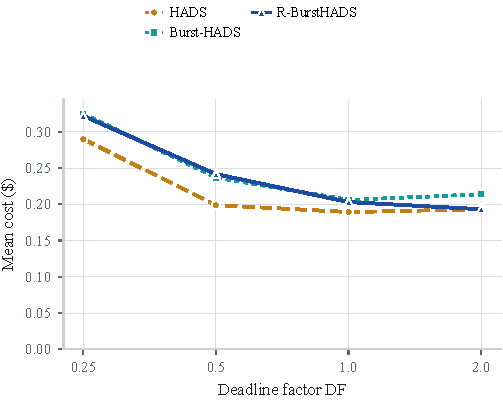
\includegraphics{fig/fig1_cost_vs_df.pdf}
  \caption{Mean cost against the deadline factor, launch limits on, 75 cells.
  Absolute dollars; the percentage changes are in Table~\ref{tab:headline}.}
  \label{fig:cost-df}
\end{figure}

\begin{figure}[t]
  \centering
  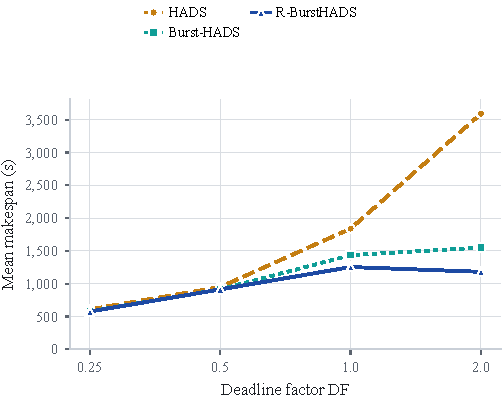
\includegraphics{fig/fig2_makespan_vs_df.pdf}
  \caption{Mean makespan against the deadline factor. R-BurstHADS's advantage
  over Burst-HADS is a wash at $\mathit{DF} = 0.5$ and grows with slack.}
  \label{fig:mk-df}
\end{figure}

\begin{figure}[t]
  \centering
  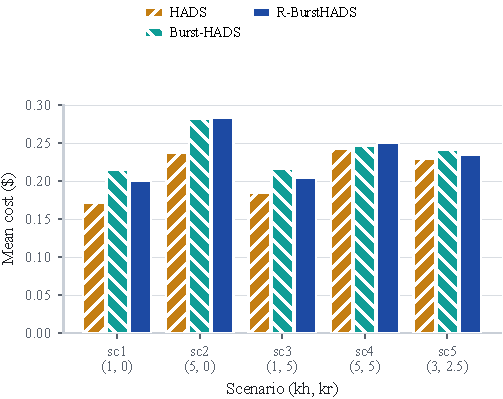
\includegraphics{fig/fig3_cost_vs_scenario.pdf}
  \caption{Mean cost by hibernation scenario $(k_h, k_r)$. The cost advantage
  over Burst-HADS is largest where interruptions are rarest.}
  \label{fig:cost-sc}
\end{figure}

\begin{figure}[t]
  \centering
  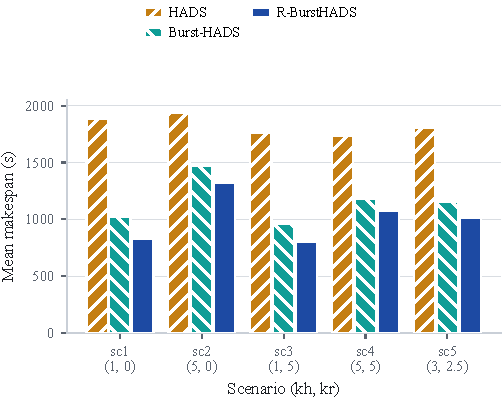
\includegraphics{fig/fig4_makespan_vs_scenario.pdf}
  \caption{Mean makespan by hibernation scenario.}
  \label{fig:mk-sc}
\end{figure}

\begin{figure}[t]
  \centering
  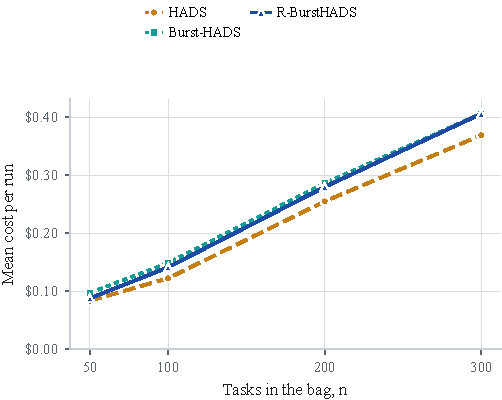
\includegraphics{fig/fig5_cost_vs_n.pdf}
  \caption{Mean cost against bag size.}
  \label{fig:cost-n}
\end{figure}

\begin{figure}[t]
  \centering
  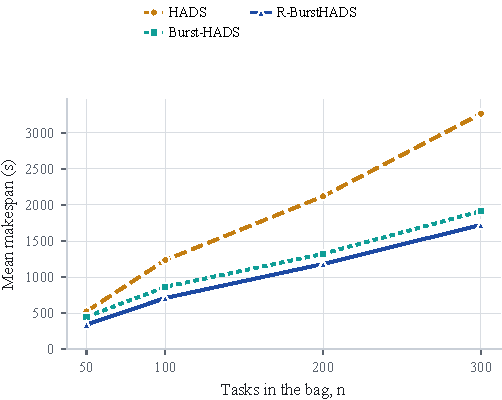
\includegraphics{fig/fig6_makespan_vs_n.pdf}
  \caption{Mean makespan against bag size.}
  \label{fig:mk-n}
\end{figure}

\section{Discussion}

\subsection{Cost--makespan trade}

Neither extension dominates HADS on cost. Over the 75 cells feasible under
launch limits, R-BurstHADS is no more expensive than HADS in 18 and Burst-HADS
in 16; the rest of the time
the makespan is bought. What the results support is a trade
priced per cell rather than a free lunch: R-BurstHADS's makespan is 25.7--29.9\%
below HADS's at every bag size, for a premium that falls from 19.0\% (the price
Burst-HADS pays) to 11.8\%. The trade is sharper against a faithful Burst-HADS:
at $\mathit{DF} = 2.0$, the one regime where that baseline both follows the
published algorithm and meets its deadlines, R-BurstHADS buys 11.0\% makespan
for 2.9\% more money, and on a small bag it pays more for no makespan gain at
all. What we can say about the difference between those regimes is that it is
utilisation rather than fleet size: the capacity R-BurstHADS provisions costs
a flat 13--15\% of the run at every bag size, but retires 33.6\% of the
core-seconds it is billed for at $|T| = 50$ against 77.8\% at $|T| = 200$.
Why it idles there we could not establish. The reading we pre-registered ---
that the guard-free primary schedule sends the work to burstables and leaves
the provisioned capacity with nothing to do --- is half confirmed and half
refuted by the data (Section~\ref{sec:results}), and we prefer to leave the
question open. A hypothesis of exactly this shape was measured and refuted
earlier in this work for a different regime, which is why we hold it to the
same standard here.

\subsection{Limitations}

The evaluation is a simulation and inherits the abstractions of its model. Five
limitations bear directly on how the numbers should be read.

First, the baselines are not a validated reproduction of the source work under
hibernation, and our Burst-HADS departs from the published algorithm in the
three ways set out in Section~\ref{sec:validation}. Every comparison here is
against those re-implementations.

Second, the cost advantage depends on launch headroom, and two thirds of it
disappears under the reference account limits.

Third, the hibernation scenarios interrupt every spot instance at the same
rate, so the per-instance-type risk differentiation that Theorem 1's trigger
reads is never exercised. No result here may be attributed to risk awareness.

Fourth, the deadline floor of 339.7\,s contains no deploy-time term, so the
five cells that sit on it generate deadlines that a scheduler charged for
instance start-up cannot always meet. They are reported separately rather than
averaged.

Fifth, the burstable tier's contribution is negative in this catalogue
(Section~\ref{sec:results}): at current on-demand prices the instance it
substitutes costs more than the one it displaces. In the source work's
catalogue the same substitution saves money, so this is a property of the price
list as much as of the algorithm.

\section{Conclusion}

We presented R-BurstHADS, which extends Burst-HADS with elastic spot
provisioning sized against the remaining deadline by a work-conservation
argument, drawing from the same instance catalogue available to the baselines.
Across 7{,}200 runs per launch-limit setting, the makespan result holds in
every aggregate we measured: 27.7\% below HADS and 12.0\% below Burst-HADS on the
full sweep, 11.0\% below an unmodified Burst-HADS at $\mathit{DF} = 2.0$, and
shorter in every other configuration measured --- limits lifted, burstable tier
disabled, hibernation switched off. Two qualifications travel with it: at
$\mathit{DF} = 0.5$ the advantage over Burst-HADS is a wash, and on the smallest
bag against an unmodified baseline it disappears. The cost result does not hold
in general. Against
the unmodified baseline R-BurstHADS is 2.9\% dearer on average, and dearer on
small bags in every configuration measured --- 12.7\% at 50 tasks and 9.6\% at
100 --- which we report as a limit of the method rather than of the
experiment. Its provisioned capacity is 33.6\% utilised at 50 tasks against
77.8\% at 200; why it idles there is measured but not explained. On the
broader sweep, against our own Burst-HADS, it is 4.6\% cheaper and dominates in
49 of 75 cells, with the three departures of that baseline disclosed and
quantified. Under launch limits Burst-HADS and R-BurstHADS miss 6 and 5 tasks
at the tightest deadlines and HADS none, though HADS has no feasible schedule
at all in 110 of those runs.

Three directions follow. The provisioning rule treats replacement instances as
equally reliable as those they replace; incorporating the replacement's own
interruption risk into (\ref{eq:sizing}) would make the sizing risk-aware as
well as deadline-aware. The pre-registered ablation indicates that the
burstable tier belongs below the on-demand fallback rather than above it, a
reordering we deliberately did not make after seeing the measurement. Finally,
the evaluation should move from a synthetic uniform workload to real BoT
traces, where the straggler tail dominates makespan and elastic rescue capacity
is likely to be worth more than reported here.

\appendices
% Generated by experiments/make_paper_tables.py -- do not edit by hand.
% Sources: DEVIATIONS.md and the committed sweeps of freeze-fix21 (2439a00d7f74).

\section{Appendix: deviation register}
\label{sec:deviations}

Every place our re-implementations differ from the published algorithms, with the status of each. The register holds 40 rows: 15 corrected, 15 design, 8 open, 1 kept, 1 inert. "Corrected" means the code now follows the source and the row is kept because earlier results used the deviation; ``design'' is a deliberate modelling choice this study keeps; ``open'' means the code still differs. The full register, with the measured effect and the evidence file behind every row, ships as supplementary material (\texttt{DEVIATIONS.md}); the three rows that bear on how the results should be read are discussed in Section~\ref{sec:validation}.

\begin{table*}[t]
\caption{The deviation register. The effect column is filled only where the effect has been measured; an em dash means it has not. The full text of every row, with its evidence file, is supplementary.}
\label{tab:deviations}
\centering
\scriptsize
\begin{tabular}{@{}lp{3.4cm}p{2.5cm}p{8.6cm}@{}}
\toprule
\# & Deviation & Status & Measured effect \\
\midrule
\multicolumn{4}{@{}l}{\textbf{Cost and billing model}} \\
\midrule
B1 & When billing starts & corrected & 20-cell cost change vs HADS +38.7 to +40.5\%; launch-to-dispatch is 5.9\% of Burst-HADS's no-hibernation cost \\
B2 & Charges while hibernated & open --- immaterial & charging EBS while hibernated: +38.7 to +37.5\%; no cell moves by 3 points \\
B3 & Billing granularity & design & 900 s quantisation: +38.7 to +30.1\%, but no-hibernation cost change +55 to +79\% \\
B4 & End of run & design & undoing fixes 2-3: +38.7 to +22.9\%, but J60 Burst-HADS no-hibernation cost \$0.165 against Table 7's \$0.112 \\
B5 & Resumed VMs that were never launched & open & 0.9-2.9\% of HADS's cost in sc3-sc5, 0\% of Burst-HADS's; removing it widens the gap to +40.7\% \\
\midrule
\multicolumn{4}{@{}l}{\textbf{Burst-HADS (TCC23, REF `IPDPS.py`)}} \\
\midrule
U1 & Planner prediction order & corrected & produced every residual deadline miss in the fixes 1-10 sweep \\
U2 & Eq 9 normaliser & corrected & with U1 fixed, removed the remaining misses \\
U3 & On-demand fallback inside the primary schedule & design --- kept, disclosed in the paper body... & fires in 905 of 2,400 runs, all at DF <= 0.5, and in all 150 floor-cell runs; over the 45 cells a reference-faithful Burst-HADS could solve, R vs Burst-HADS is -19.1\% makespan and -7.5\% cost \\
U4 & Planner checkpoint overhead & corrected & all of HADS's deadline misses before fix 8 \\
U5 & Proactive burstable allocation guard & kept --- an ADDITION to the published algorit... & R vs Burst-HADS -4.62\% cost as frozen against +2.45\% with TCC23 3.2 followed in full; removing the guard turns 974 clean Burst-HADS runs into missing ones, against 0 the other way \\
U6 & Migration candidates & corrected & hibernation makespan reduction 14.7 to 21.5\%, 20-cell cost change +38.7 to +16.0\% \\
U7 & ILS relaxation & design & --- \\
U8 & Infeasibility score & design & the reference's +inf sentinel gives near-identical results \\
U9 & Deployment overhead ω & design & --- \\
U10 & Checkpoint overhead in Attempt 3's deadline test & inert --- fix 20 & changes 0 of 7,200 runs, alone and within the combined set \\
U11 & Attempt 3's candidate loop & open & exposure 1,455 Burst-HADS and 759 R-BurstHADS mid-run launches; the effect of restricting the loop is unmeasured \\
U12 & Algorithm 1 Part 2, step 2: violators the burstables did not take & open --- measured and disclosed & 575 of 2,400 runs leave 12,150 violators on spot; implementing it alone takes Burst-HADS from 6 to 302 missed tasks and 4.1 points dearer against HADS, and changes nothing on TCC23's catalogue \\
\midrule
\multicolumn{4}{@{}l}{\textbf{HADS (CC21, REF `CCScheduler.py`)}} \\
\midrule
H1 & Queue packing & design & --- \\
H2 & Migration candidates & corrected & HADS launches 7.95 to 5.11 spot VMs per run and is 2.6\% dearer and 3.5\% slower against itself \\
H3 & Work stealing & design & --- \\
H4 & Planner checkpoint overhead & corrected & as U4 \\
\midrule
\multicolumn{4}{@{}l}{\textbf{Environment, catalogue and workload}} \\
\midrule
E1 & Instance limits & corrected & infeasible runs 250/250/250 to 5/0/0; missed tasks 2,533/1,981/1,090 to 0/0/43 \\
E2 & Migration at a spent limit & design & fires in 23 of 7,200 runs, all at DF 0.25, one in a headline cell; 0 launches forced past a limit \\
E3 & On-demand template when all on-demand VMs have terminated & corrected & 0.1 launches per run; not separable from E1, adopted in the same commit \\
E4 & Spot pool size & design --- 3 kept & J60 makespan change vs HADS -71\% at 3 spot copies, -78\% at 5; Burst-HADS's hibernation premium +94/+47/+62\% at 3/2/1 \\
E5 & Job generator (validation) & design & both job generators reported side by side \\
E6 & Hibernation process & open & see B5 \\
E8 & Hibernations suffered per run & open --- pool size is the owner's decision & our runs see 1.3-3.6x TCC23's hibernations per run, flat across jobs \\
E7 & Per-core speed & design --- kept & a burst-mode task costs 1.15x a lone task on fresh on-demand in the sweep catalogue, 0.83x in TCC23's \\
E9 & Burstable baseline performance & design --- recorded & --- \\
E10 & Allocation Cycle boundaries & corrected & Burst-HADS's hibernation premium +42 to +39\%; sweep mean cost HADS -4.5\%, Burst-HADS -2.2\%, R-BurstHADS -2.9\% \\
E11 & Progress credited at a checkpoint & corrected & runs changed 1,472/1,769/1,531 of 2,400; R vs Burst-HADS cost -5.39 to -5.30\% \\
E12 & Deploy time of VMs a scheduler launches & corrected & 36,574 of 42,249 launches started a task early before the fix; 0 of 42,623 after \\
E13 & Remaining work in hibernation rescue tests & open & exposure 17.4/25.2/27.9 displaced running tasks per run; effect unmeasured \\
E14 & Deadline floor & design & HADS infeasible in 110 of the 150 floor-cell runs, against 10 before deploy time was charged; every one feasible with limits off \\
\midrule
\multicolumn{4}{@{}l}{\textbf{R-BurstHADS (this study's scheduler)}} \\
\midrule
R1 & Deadline test in the saturation re-placement & corrected & 108 of the 109 misses at freeze-round-b; fix 17a took them 109 to 1 \\
R2 & Saturation response with no launch room & open --- measured and rejected & fix 17b: misses 109 to 1 but 337 of 2,400 runs change and dominance 44 to 43; rejected \\
R3 & When the saturation response fires & design --- code kept & fix 17c: misses 109 to 73, 282 runs change; rejected \\
R4 & Boot delay of VMs R-BurstHADS provisions & corrected & 6,661 early starts in 1,276 of 2,400 runs; R vs Burst-HADS cost -5.39 to -4.96\% \\
R5 & Burstables R-BurstHADS launches mid-run & corrected & the branch still fires after the fix: 1,453 tier-3 burstables in 2,400 runs, against 1,477 before \\
\bottomrule
\end{tabular}
\end{table*}

\section{Appendix: per-cell results}
\label{sec:percell}

These are the cell means behind every aggregate in Section~\ref{sec:results}: Table~\ref{tab:cells-on} under the reference account limits and Table~\ref{tab:cells-off} without them.

\begin{longtable}{@{}lrrrrrrrr@{}}
\caption{Per-cell means with 95\% confidence intervals, launch limits on. Makespan in seconds, cost in dollars; each cell is 30 seeds. A cell in which a scheduler was infeasible in some seed is averaged over its feasible seeds and excluded from the cross-scheduler tables (Section~\ref{sec:results}).}\label{tab:cells-on}\\
\toprule
Scenario & $|T|$ & DF & \multicolumn{2}{c}{HADS} & \multicolumn{2}{c}{Burst-HADS} & \multicolumn{2}{c}{R-BurstHADS} \\
 & & & mkp & cost & mkp & cost & mkp & cost \\
\midrule
\endfirsthead
\toprule
Scenario & $|T|$ & DF & \multicolumn{2}{c}{HADS} & \multicolumn{2}{c}{Burst-HADS} & \multicolumn{2}{c}{R-BurstHADS} \\
 & & & mkp & cost & mkp & cost & mkp & cost \\
\midrule
\endhead
\bottomrule
\endfoot
sc1 & 50 & 0.25 & 335\,$\pm$1 & 0.106\,$\pm$0.004 & 247\,$\pm$7 & 0.101\,$\pm$0.004 & 243\,$\pm$6 & 0.103\,$\pm$0.005 \\
sc1 & 50 & 0.5 & 335\,$\pm$1 & 0.106\,$\pm$0.004 & 247\,$\pm$7 & 0.101\,$\pm$0.004 & 243\,$\pm$6 & 0.103\,$\pm$0.005 \\
sc1 & 50 & 1.0 & 491\,$\pm$26 & 0.042\,$\pm$0.003 & 496\,$\pm$40 & 0.068\,$\pm$0.005 & 309\,$\pm$19 & 0.055\,$\pm$0.002 \\
sc1 & 50 & 2.0 & 1,035\,$\pm$34 & 0.041\,$\pm$0.005 & 583\,$\pm$110 & 0.089\,$\pm$0.014 & 288\,$\pm$8 & 0.057\,$\pm$0.002 \\
sc1 & 100 & 0.25 & 339\,$\pm$0 & 0.210\,$\pm$0.006 & 329\,$\pm$4 & 0.230\,$\pm$0.007 & 328\,$\pm$5 & 0.231\,$\pm$0.007 \\
sc1 & 100 & 0.5 & 581\,$\pm$7 & 0.115\,$\pm$0.004 & 552\,$\pm$14 & 0.145\,$\pm$0.006 & 502\,$\pm$28 & 0.137\,$\pm$0.008 \\
sc1 & 100 & 1.0 & 1,143\,$\pm$25 & 0.087\,$\pm$0.007 & 877\,$\pm$77 & 0.118\,$\pm$0.006 & 582\,$\pm$61 & 0.102\,$\pm$0.005 \\
sc1 & 100 & 2.0 & 2,256\,$\pm$39 & 0.082\,$\pm$0.010 & 853\,$\pm$123 & 0.132\,$\pm$0.012 & 513\,$\pm$49 & 0.105\,$\pm$0.005 \\
sc1 & 200 & 0.25 & 596\,$\pm$1 & 0.297\,$\pm$0.006 & 586\,$\pm$4 & 0.340\,$\pm$0.005 & 574\,$\pm$8 & 0.334\,$\pm$0.006 \\
sc1 & 200 & 0.5 & 1,177\,$\pm$15 & 0.183\,$\pm$0.011 & 1,152\,$\pm$13 & 0.234\,$\pm$0.011 & 1,090\,$\pm$42 & 0.213\,$\pm$0.018 \\
sc1 & 200 & 1.0 & 2,357\,$\pm$23 & 0.177\,$\pm$0.014 & 1,564\,$\pm$139 & 0.222\,$\pm$0.013 & 1,186\,$\pm$104 & 0.195\,$\pm$0.009 \\
sc1 & 200 & 2.0 & 4,640\,$\pm$48 & 0.160\,$\pm$0.019 & 1,462\,$\pm$100 & 0.243\,$\pm$0.014 & 1,116\,$\pm$77 & 0.207\,$\pm$0.011 \\
sc1 & 300 & 0.25 & 896\,$\pm$1 & 0.398\,$\pm$0.007 & 884\,$\pm$4 & 0.472\,$\pm$0.006 & 882\,$\pm$6 & 0.467\,$\pm$0.009 \\
sc1 & 300 & 0.5 & 1,784\,$\pm$12 & 0.272\,$\pm$0.015 & 1,717\,$\pm$26 & 0.335\,$\pm$0.015 & 1,649\,$\pm$66 & 0.306\,$\pm$0.022 \\
sc1 & 300 & 1.0 & 3,552\,$\pm$24 & 0.265\,$\pm$0.024 & 2,132\,$\pm$154 & 0.300\,$\pm$0.011 & 1,663\,$\pm$127 & 0.295\,$\pm$0.015 \\
sc1 & 300 & 2.0 & 7,022\,$\pm$57 & 0.232\,$\pm$0.027 & 1,940\,$\pm$96 & 0.326\,$\pm$0.015 & 1,582\,$\pm$119 & 0.325\,$\pm$0.020 \\
sc2 & 50 & 0.25 & 336\,$\pm$1 & 0.104\,$\pm$0.005 & 313\,$\pm$7 & 0.111\,$\pm$0.005 & 304\,$\pm$11 & 0.109\,$\pm$0.005 \\
sc2 & 50 & 0.5 & 336\,$\pm$1 & 0.104\,$\pm$0.005 & 313\,$\pm$7 & 0.111\,$\pm$0.005 & 304\,$\pm$11 & 0.109\,$\pm$0.005 \\
sc2 & 50 & 1.0 & 594\,$\pm$2 & 0.068\,$\pm$0.004 & 569\,$\pm$9 & 0.087\,$\pm$0.004 & 565\,$\pm$24 & 0.092\,$\pm$0.008 \\
sc2 & 50 & 2.0 & 1,184\,$\pm$6 & 0.069\,$\pm$0.004 & 931\,$\pm$82 & 0.090\,$\pm$0.008 & 596\,$\pm$131 & 0.075\,$\pm$0.012 \\
sc2 & 100 & 0.25 & 339\,$\pm$0 & 0.207\,$\pm$0.007 & 339\,$\pm$1 & 0.219\,$\pm$0.006 & 338\,$\pm$1 & 0.220\,$\pm$0.006 \\
sc2 & 100 & 0.5 & 597\,$\pm$0 & 0.145\,$\pm$0.005 & 589\,$\pm$3 & 0.188\,$\pm$0.005 & 592\,$\pm$2 & 0.189\,$\pm$0.006 \\
sc2 & 100 & 1.0 & 1,194\,$\pm$1 & 0.142\,$\pm$0.009 & 1,137\,$\pm$20 & 0.167\,$\pm$0.009 & 1,142\,$\pm$47 & 0.180\,$\pm$0.017 \\
sc2 & 100 & 2.0 & 2,385\,$\pm$3 & 0.134\,$\pm$0.006 & 1,521\,$\pm$143 & 0.158\,$\pm$0.014 & 1,099\,$\pm$233 & 0.141\,$\pm$0.023 \\
sc2 & 200 & 0.25 & 598\,$\pm$0 & 0.332\,$\pm$0.008 & 596\,$\pm$1 & 0.380\,$\pm$0.007 & 597\,$\pm$1 & 0.376\,$\pm$0.009 \\
sc2 & 200 & 0.5 & 1,196\,$\pm$0 & 0.275\,$\pm$0.007 & 1,184\,$\pm$5 & 0.335\,$\pm$0.008 & 1,190\,$\pm$2 & 0.361\,$\pm$0.014 \\
sc2 & 200 & 1.0 & 2,390\,$\pm$1 & 0.278\,$\pm$0.013 & 2,286\,$\pm$32 & 0.335\,$\pm$0.020 & 2,233\,$\pm$120 & 0.349\,$\pm$0.035 \\
sc2 & 200 & 2.0 & 4,783\,$\pm$1 & 0.256\,$\pm$0.012 & 2,623\,$\pm$341 & 0.293\,$\pm$0.028 & 2,110\,$\pm$493 & 0.281\,$\pm$0.047 \\
sc2 & 300 & 0.25 & 897\,$\pm$0 & 0.477\,$\pm$0.009 & 895\,$\pm$1 & 0.553\,$\pm$0.008 & 895\,$\pm$1 & 0.543\,$\pm$0.010 \\
sc2 & 300 & 0.5 & 1,793\,$\pm$1 & 0.406\,$\pm$0.007 & 1,765\,$\pm$8 & 0.494\,$\pm$0.009 & 1,788\,$\pm$2 & 0.532\,$\pm$0.019 \\
sc2 & 300 & 1.0 & 3,588\,$\pm$1 & 0.399\,$\pm$0.015 & 3,417\,$\pm$60 & 0.496\,$\pm$0.025 & 3,312\,$\pm$210 & 0.504\,$\pm$0.048 \\
sc2 & 300 & 2.0 & 7,175\,$\pm$2 & 0.378\,$\pm$0.016 & 3,936\,$\pm$506 & 0.431\,$\pm$0.037 & 3,123\,$\pm$753 & 0.407\,$\pm$0.068 \\
sc3 & 50 & 0.25 & 330\,$\pm$4 & 0.116\,$\pm$0.004 & 246\,$\pm$8 & 0.107\,$\pm$0.007 & 243\,$\pm$6 & 0.109\,$\pm$0.006 \\
sc3 & 50 & 0.5 & 330\,$\pm$4 & 0.116\,$\pm$0.004 & 246\,$\pm$8 & 0.107\,$\pm$0.007 & 243\,$\pm$6 & 0.109\,$\pm$0.006 \\
sc3 & 50 & 1.0 & 418\,$\pm$8 & 0.043\,$\pm$0.002 & 463\,$\pm$40 & 0.075\,$\pm$0.007 & 293\,$\pm$9 & 0.057\,$\pm$0.002 \\
sc3 & 50 & 2.0 & 883\,$\pm$27 & 0.055\,$\pm$0.005 & 544\,$\pm$113 & 0.091\,$\pm$0.018 & 288\,$\pm$9 & 0.058\,$\pm$0.002 \\
sc3 & 100 & 0.25 & 337\,$\pm$3 & 0.222\,$\pm$0.007 & 328\,$\pm$4 & 0.236\,$\pm$0.007 & 325\,$\pm$5 & 0.237\,$\pm$0.008 \\
sc3 & 100 & 0.5 & 517\,$\pm$18 & 0.113\,$\pm$0.006 & 532\,$\pm$19 & 0.150\,$\pm$0.007 & 486\,$\pm$27 & 0.144\,$\pm$0.008 \\
sc3 & 100 & 1.0 & 1,012\,$\pm$10 & 0.093\,$\pm$0.006 & 759\,$\pm$74 & 0.121\,$\pm$0.009 & 559\,$\pm$50 & 0.108\,$\pm$0.008 \\
sc3 & 100 & 2.0 & 2,044\,$\pm$52 & 0.114\,$\pm$0.011 & 762\,$\pm$95 & 0.129\,$\pm$0.012 & 528\,$\pm$72 & 0.109\,$\pm$0.008 \\
sc3 & 200 & 0.25 & 595\,$\pm$2 & 0.311\,$\pm$0.005 & 572\,$\pm$6 & 0.346\,$\pm$0.006 & 558\,$\pm$10 & 0.340\,$\pm$0.007 \\
sc3 & 200 & 0.5 & 1,068\,$\pm$21 & 0.168\,$\pm$0.010 & 1,078\,$\pm$29 & 0.221\,$\pm$0.009 & 1,027\,$\pm$44 & 0.202\,$\pm$0.014 \\
sc3 & 200 & 1.0 & 2,235\,$\pm$29 & 0.195\,$\pm$0.014 & 1,378\,$\pm$106 & 0.220\,$\pm$0.015 & 1,096\,$\pm$54 & 0.196\,$\pm$0.006 \\
sc3 & 200 & 2.0 & 4,302\,$\pm$94 & 0.203\,$\pm$0.022 & 1,437\,$\pm$111 & 0.244\,$\pm$0.018 & 1,095\,$\pm$58 & 0.207\,$\pm$0.008 \\
sc3 & 300 & 0.25 & 894\,$\pm$2 & 0.416\,$\pm$0.008 & 868\,$\pm$9 & 0.478\,$\pm$0.009 & 864\,$\pm$12 & 0.476\,$\pm$0.010 \\
sc3 & 300 & 0.5 & 1,685\,$\pm$24 & 0.255\,$\pm$0.015 & 1,641\,$\pm$40 & 0.320\,$\pm$0.015 & 1,567\,$\pm$65 & 0.306\,$\pm$0.015 \\
sc3 & 300 & 1.0 & 3,450\,$\pm$27 & 0.284\,$\pm$0.021 & 1,918\,$\pm$103 & 0.299\,$\pm$0.009 & 1,636\,$\pm$97 & 0.311\,$\pm$0.014 \\
sc3 & 300 & 2.0 & 6,653\,$\pm$136 & 0.285\,$\pm$0.031 & 2,000\,$\pm$105 & 0.333\,$\pm$0.014 & 1,607\,$\pm$121 & 0.334\,$\pm$0.021 \\
sc4 & 50 & 0.25 & 327\,$\pm$4 & 0.116\,$\pm$0.005 & 275\,$\pm$10 & 0.107\,$\pm$0.005 & 262\,$\pm$9 & 0.105\,$\pm$0.005 \\
sc4 & 50 & 0.5 & 327\,$\pm$4 & 0.116\,$\pm$0.005 & 275\,$\pm$10 & 0.107\,$\pm$0.005 & 262\,$\pm$9 & 0.105\,$\pm$0.005 \\
sc4 & 50 & 1.0 & 446\,$\pm$15 & 0.057\,$\pm$0.005 & 494\,$\pm$30 & 0.079\,$\pm$0.008 & 472\,$\pm$43 & 0.080\,$\pm$0.011 \\
sc4 & 50 & 2.0 & 755\,$\pm$23 & 0.063\,$\pm$0.004 & 875\,$\pm$65 & 0.116\,$\pm$0.010 & 465\,$\pm$94 & 0.074\,$\pm$0.014 \\
sc4 & 100 & 0.25 & 335\,$\pm$4 & 0.222\,$\pm$0.005 & 339\,$\pm$4 & 0.234\,$\pm$0.008 & 339\,$\pm$4 & 0.235\,$\pm$0.009 \\
sc4 & 100 & 0.5 & 560\,$\pm$10 & 0.138\,$\pm$0.008 & 557\,$\pm$15 & 0.176\,$\pm$0.008 & 575\,$\pm$15 & 0.184\,$\pm$0.011 \\
sc4 & 100 & 1.0 & 978\,$\pm$28 & 0.129\,$\pm$0.011 & 981\,$\pm$55 & 0.141\,$\pm$0.013 & 972\,$\pm$83 & 0.154\,$\pm$0.018 \\
sc4 & 100 & 2.0 & 1,691\,$\pm$54 & 0.144\,$\pm$0.008 & 1,234\,$\pm$118 & 0.159\,$\pm$0.013 & 913\,$\pm$170 & 0.145\,$\pm$0.024 \\
sc4 & 200 & 0.25 & 596\,$\pm$2 & 0.328\,$\pm$0.009 & 585\,$\pm$4 & 0.371\,$\pm$0.009 & 590\,$\pm$3 & 0.371\,$\pm$0.010 \\
sc4 & 200 & 0.5 & 1,115\,$\pm$24 & 0.241\,$\pm$0.014 & 1,100\,$\pm$30 & 0.292\,$\pm$0.013 & 1,187\,$\pm$4 & 0.331\,$\pm$0.018 \\
sc4 & 200 & 1.0 & 2,164\,$\pm$51 & 0.282\,$\pm$0.017 & 1,777\,$\pm$98 & 0.243\,$\pm$0.015 & 1,668\,$\pm$186 & 0.257\,$\pm$0.034 \\
sc4 & 200 & 2.0 & 4,120\,$\pm$108 & 0.307\,$\pm$0.015 & 1,844\,$\pm$114 & 0.256\,$\pm$0.012 & 1,562\,$\pm$261 & 0.245\,$\pm$0.033 \\
sc4 & 300 & 0.25 & 895\,$\pm$1 & 0.459\,$\pm$0.013 & 872\,$\pm$6 & 0.522\,$\pm$0.012 & 890\,$\pm$4 & 0.527\,$\pm$0.015 \\
sc4 & 300 & 0.5 & 1,741\,$\pm$18 & 0.375\,$\pm$0.021 & 1,662\,$\pm$34 & 0.435\,$\pm$0.018 & 1,782\,$\pm$5 & 0.480\,$\pm$0.027 \\
sc4 & 300 & 1.0 & 3,476\,$\pm$42 & 0.430\,$\pm$0.022 & 2,673\,$\pm$121 & 0.355\,$\pm$0.022 & 2,332\,$\pm$235 & 0.348\,$\pm$0.042 \\
sc4 & 300 & 2.0 & 6,763\,$\pm$91 & 0.449\,$\pm$0.018 & 2,446\,$\pm$183 & 0.345\,$\pm$0.019 & 2,119\,$\pm$379 & 0.343\,$\pm$0.048 \\
sc5 & 50 & 0.25 & 332\,$\pm$3 & 0.115\,$\pm$0.004 & 273\,$\pm$11 & 0.108\,$\pm$0.006 & 260\,$\pm$8 & 0.105\,$\pm$0.005 \\
sc5 & 50 & 0.5 & 332\,$\pm$3 & 0.115\,$\pm$0.004 & 273\,$\pm$11 & 0.108\,$\pm$0.006 & 260\,$\pm$8 & 0.105\,$\pm$0.005 \\
sc5 & 50 & 1.0 & 486\,$\pm$25 & 0.057\,$\pm$0.006 & 493\,$\pm$26 & 0.075\,$\pm$0.005 & 453\,$\pm$48 & 0.075\,$\pm$0.009 \\
sc5 & 50 & 2.0 & 865\,$\pm$45 & 0.064\,$\pm$0.007 & 792\,$\pm$90 & 0.104\,$\pm$0.011 & 448\,$\pm$98 & 0.070\,$\pm$0.010 \\
sc5 & 100 & 0.25 & 337\,$\pm$3 & 0.222\,$\pm$0.008 & 337\,$\pm$4 & 0.231\,$\pm$0.007 & 336\,$\pm$4 & 0.232\,$\pm$0.007 \\
sc5 & 100 & 0.5 & 572\,$\pm$12 & 0.134\,$\pm$0.009 & 554\,$\pm$11 & 0.168\,$\pm$0.008 & 564\,$\pm$17 & 0.169\,$\pm$0.012 \\
sc5 & 100 & 1.0 & 1,042\,$\pm$28 & 0.121\,$\pm$0.012 & 954\,$\pm$67 & 0.132\,$\pm$0.012 & 832\,$\pm$94 & 0.130\,$\pm$0.016 \\
sc5 & 100 & 2.0 & 1,958\,$\pm$60 & 0.144\,$\pm$0.011 & 1,120\,$\pm$119 & 0.146\,$\pm$0.012 & 789\,$\pm$146 & 0.124\,$\pm$0.013 \\
sc5 & 200 & 0.25 & 596\,$\pm$1 & 0.322\,$\pm$0.009 & 584\,$\pm$5 & 0.363\,$\pm$0.009 & 581\,$\pm$6 & 0.357\,$\pm$0.011 \\
sc5 & 200 & 0.5 & 1,159\,$\pm$17 & 0.241\,$\pm$0.014 & 1,115\,$\pm$22 & 0.284\,$\pm$0.014 & 1,181\,$\pm$8 & 0.308\,$\pm$0.023 \\
sc5 & 200 & 1.0 & 2,280\,$\pm$41 & 0.259\,$\pm$0.022 & 1,844\,$\pm$121 & 0.249\,$\pm$0.019 & 1,595\,$\pm$174 & 0.240\,$\pm$0.026 \\
sc5 & 200 & 2.0 & 4,460\,$\pm$99 & 0.279\,$\pm$0.020 & 1,721\,$\pm$159 & 0.246\,$\pm$0.015 & 1,408\,$\pm$164 & 0.224\,$\pm$0.014 \\
sc5 & 300 & 0.25 & 896\,$\pm$1 & 0.450\,$\pm$0.015 & 880\,$\pm$8 & 0.517\,$\pm$0.013 & 886\,$\pm$5 & 0.507\,$\pm$0.016 \\
sc5 & 300 & 0.5 & 1,770\,$\pm$18 & 0.361\,$\pm$0.019 & 1,709\,$\pm$32 & 0.425\,$\pm$0.021 & 1,760\,$\pm$32 & 0.440\,$\pm$0.037 \\
sc5 & 300 & 1.0 & 3,510\,$\pm$38 & 0.380\,$\pm$0.028 & 2,519\,$\pm$157 & 0.338\,$\pm$0.024 & 2,175\,$\pm$239 & 0.336\,$\pm$0.039 \\
sc5 & 300 & 2.0 & 6,882\,$\pm$121 & 0.404\,$\pm$0.031 & 2,424\,$\pm$231 & 0.345\,$\pm$0.021 & 1,969\,$\pm$159 & 0.333\,$\pm$0.015 \\
\end{longtable}

\begin{longtable}{@{}lrrrrrrrr@{}}
\caption{Per-cell means with 95\% confidence intervals, launch limits off. Makespan in seconds, cost in dollars; each cell is 30 seeds. A cell in which a scheduler was infeasible in some seed is averaged over its feasible seeds and excluded from the cross-scheduler tables (Section~\ref{sec:results}).}\label{tab:cells-off}\\
\toprule
Scenario & $|T|$ & DF & \multicolumn{2}{c}{HADS} & \multicolumn{2}{c}{Burst-HADS} & \multicolumn{2}{c}{R-BurstHADS} \\
 & & & mkp & cost & mkp & cost & mkp & cost \\
\midrule
\endfirsthead
\toprule
Scenario & $|T|$ & DF & \multicolumn{2}{c}{HADS} & \multicolumn{2}{c}{Burst-HADS} & \multicolumn{2}{c}{R-BurstHADS} \\
 & & & mkp & cost & mkp & cost & mkp & cost \\
\midrule
\endhead
\bottomrule
\endfoot
sc1 & 50 & 0.25 & 336\,$\pm$1 & 0.101\,$\pm$0.003 & 249\,$\pm$9 & 0.100\,$\pm$0.004 & 244\,$\pm$8 & 0.102\,$\pm$0.005 \\
sc1 & 50 & 0.5 & 336\,$\pm$1 & 0.101\,$\pm$0.003 & 249\,$\pm$9 & 0.100\,$\pm$0.004 & 244\,$\pm$8 & 0.102\,$\pm$0.005 \\
sc1 & 50 & 1.0 & 491\,$\pm$26 & 0.042\,$\pm$0.003 & 496\,$\pm$40 & 0.068\,$\pm$0.005 & 301\,$\pm$21 & 0.056\,$\pm$0.002 \\
sc1 & 50 & 2.0 & 1,035\,$\pm$34 & 0.041\,$\pm$0.005 & 583\,$\pm$110 & 0.089\,$\pm$0.014 & 284\,$\pm$8 & 0.059\,$\pm$0.002 \\
sc1 & 100 & 0.25 & 338\,$\pm$0 & 0.200\,$\pm$0.005 & 331\,$\pm$4 & 0.224\,$\pm$0.007 & 330\,$\pm$4 & 0.226\,$\pm$0.007 \\
sc1 & 100 & 0.5 & 581\,$\pm$7 & 0.115\,$\pm$0.004 & 552\,$\pm$14 & 0.145\,$\pm$0.006 & 455\,$\pm$22 & 0.130\,$\pm$0.006 \\
sc1 & 100 & 1.0 & 1,143\,$\pm$25 & 0.087\,$\pm$0.007 & 877\,$\pm$77 & 0.118\,$\pm$0.006 & 533\,$\pm$49 & 0.103\,$\pm$0.004 \\
sc1 & 100 & 2.0 & 2,256\,$\pm$39 & 0.082\,$\pm$0.010 & 853\,$\pm$123 & 0.132\,$\pm$0.012 & 492\,$\pm$36 & 0.110\,$\pm$0.006 \\
sc1 & 200 & 0.25 & 597\,$\pm$1 & 0.287\,$\pm$0.004 & 589\,$\pm$3 & 0.346\,$\pm$0.005 & 573\,$\pm$7 & 0.343\,$\pm$0.005 \\
sc1 & 200 & 0.5 & 1,177\,$\pm$15 & 0.180\,$\pm$0.009 & 1,152\,$\pm$13 & 0.234\,$\pm$0.011 & 1,047\,$\pm$45 & 0.183\,$\pm$0.004 \\
sc1 & 200 & 1.0 & 2,357\,$\pm$23 & 0.177\,$\pm$0.014 & 1,564\,$\pm$139 & 0.222\,$\pm$0.013 & 1,054\,$\pm$52 & 0.195\,$\pm$0.006 \\
sc1 & 200 & 2.0 & 4,640\,$\pm$48 & 0.160\,$\pm$0.019 & 1,462\,$\pm$100 & 0.243\,$\pm$0.014 & 1,131\,$\pm$85 & 0.220\,$\pm$0.011 \\
sc1 & 300 & 0.25 & 896\,$\pm$1 & 0.393\,$\pm$0.006 & 890\,$\pm$2 & 0.468\,$\pm$0.006 & 877\,$\pm$8 & 0.451\,$\pm$0.007 \\
sc1 & 300 & 0.5 & 1,784\,$\pm$12 & 0.271\,$\pm$0.015 & 1,717\,$\pm$26 & 0.335\,$\pm$0.015 & 1,620\,$\pm$69 & 0.286\,$\pm$0.013 \\
sc1 & 300 & 1.0 & 3,552\,$\pm$24 & 0.264\,$\pm$0.023 & 2,132\,$\pm$154 & 0.300\,$\pm$0.011 & 1,510\,$\pm$96 & 0.297\,$\pm$0.016 \\
sc1 & 300 & 2.0 & 7,022\,$\pm$57 & 0.232\,$\pm$0.027 & 1,940\,$\pm$96 & 0.326\,$\pm$0.015 & 1,472\,$\pm$103 & 0.329\,$\pm$0.020 \\
sc2 & 50 & 0.25 & 336\,$\pm$1 & 0.099\,$\pm$0.003 & 313\,$\pm$7 & 0.108\,$\pm$0.004 & 303\,$\pm$12 & 0.106\,$\pm$0.004 \\
sc2 & 50 & 0.5 & 336\,$\pm$1 & 0.099\,$\pm$0.003 & 313\,$\pm$7 & 0.108\,$\pm$0.004 & 303\,$\pm$12 & 0.106\,$\pm$0.004 \\
sc2 & 50 & 1.0 & 594\,$\pm$2 & 0.066\,$\pm$0.003 & 569\,$\pm$9 & 0.087\,$\pm$0.004 & 536\,$\pm$28 & 0.072\,$\pm$0.006 \\
sc2 & 50 & 2.0 & 1,184\,$\pm$6 & 0.069\,$\pm$0.004 & 931\,$\pm$82 & 0.090\,$\pm$0.008 & 540\,$\pm$121 & 0.066\,$\pm$0.007 \\
sc2 & 100 & 0.25 & 338\,$\pm$0 & 0.198\,$\pm$0.005 & 339\,$\pm$1 & 0.212\,$\pm$0.005 & 339\,$\pm$1 & 0.214\,$\pm$0.006 \\
sc2 & 100 & 0.5 & 598\,$\pm$0 & 0.141\,$\pm$0.005 & 591\,$\pm$3 & 0.183\,$\pm$0.004 & 588\,$\pm$4 & 0.167\,$\pm$0.006 \\
sc2 & 100 & 1.0 & 1,194\,$\pm$1 & 0.135\,$\pm$0.006 & 1,137\,$\pm$20 & 0.167\,$\pm$0.009 & 1,019\,$\pm$76 & 0.112\,$\pm$0.004 \\
sc2 & 100 & 2.0 & 2,385\,$\pm$3 & 0.134\,$\pm$0.006 & 1,521\,$\pm$143 & 0.158\,$\pm$0.014 & 846\,$\pm$169 & 0.118\,$\pm$0.010 \\
sc2 & 200 & 0.25 & 598\,$\pm$0 & 0.310\,$\pm$0.005 & 597\,$\pm$0 & 0.372\,$\pm$0.005 & 595\,$\pm$1 & 0.362\,$\pm$0.008 \\
sc2 & 200 & 0.5 & 1,196\,$\pm$0 & 0.269\,$\pm$0.007 & 1,188\,$\pm$3 & 0.333\,$\pm$0.008 & 1,162\,$\pm$12 & 0.203\,$\pm$0.005 \\
sc2 & 200 & 1.0 & 2,390\,$\pm$1 & 0.267\,$\pm$0.009 & 2,286\,$\pm$32 & 0.335\,$\pm$0.020 & 2,027\,$\pm$165 & 0.220\,$\pm$0.010 \\
sc2 & 200 & 2.0 & 4,783\,$\pm$1 & 0.256\,$\pm$0.012 & 2,623\,$\pm$341 & 0.293\,$\pm$0.028 & 1,664\,$\pm$280 & 0.226\,$\pm$0.014 \\
sc2 & 300 & 0.25 & 897\,$\pm$0 & 0.449\,$\pm$0.006 & 895\,$\pm$1 & 0.525\,$\pm$0.007 & 894\,$\pm$1 & 0.461\,$\pm$0.005 \\
sc2 & 300 & 0.5 & 1,794\,$\pm$1 & 0.399\,$\pm$0.009 & 1,783\,$\pm$5 & 0.491\,$\pm$0.010 & 1,745\,$\pm$18 & 0.276\,$\pm$0.005 \\
sc2 & 300 & 1.0 & 3,588\,$\pm$1 & 0.392\,$\pm$0.012 & 3,417\,$\pm$60 & 0.496\,$\pm$0.025 & 3,065\,$\pm$234 & 0.320\,$\pm$0.008 \\
sc2 & 300 & 2.0 & 7,175\,$\pm$2 & 0.378\,$\pm$0.016 & 3,936\,$\pm$506 & 0.431\,$\pm$0.037 & 2,223\,$\pm$344 & 0.329\,$\pm$0.020 \\
sc3 & 50 & 0.25 & 332\,$\pm$3 & 0.112\,$\pm$0.003 & 247\,$\pm$9 & 0.104\,$\pm$0.006 & 243\,$\pm$9 & 0.107\,$\pm$0.006 \\
sc3 & 50 & 0.5 & 332\,$\pm$3 & 0.112\,$\pm$0.003 & 247\,$\pm$9 & 0.104\,$\pm$0.006 & 243\,$\pm$9 & 0.107\,$\pm$0.006 \\
sc3 & 50 & 1.0 & 418\,$\pm$8 & 0.043\,$\pm$0.002 & 463\,$\pm$40 & 0.075\,$\pm$0.007 & 285\,$\pm$12 & 0.058\,$\pm$0.002 \\
sc3 & 50 & 2.0 & 883\,$\pm$27 & 0.055\,$\pm$0.005 & 544\,$\pm$113 & 0.091\,$\pm$0.018 & 284\,$\pm$9 & 0.059\,$\pm$0.002 \\
sc3 & 100 & 0.25 & 338\,$\pm$1 & 0.211\,$\pm$0.005 & 326\,$\pm$4 & 0.229\,$\pm$0.007 & 323\,$\pm$7 & 0.231\,$\pm$0.008 \\
sc3 & 100 & 0.5 & 517\,$\pm$18 & 0.113\,$\pm$0.006 & 532\,$\pm$19 & 0.150\,$\pm$0.007 & 460\,$\pm$26 & 0.143\,$\pm$0.008 \\
sc3 & 100 & 1.0 & 1,012\,$\pm$10 & 0.093\,$\pm$0.006 & 759\,$\pm$74 & 0.121\,$\pm$0.009 & 522\,$\pm$49 & 0.108\,$\pm$0.007 \\
sc3 & 100 & 2.0 & 2,044\,$\pm$52 & 0.114\,$\pm$0.011 & 762\,$\pm$95 & 0.129\,$\pm$0.012 & 504\,$\pm$66 & 0.111\,$\pm$0.007 \\
sc3 & 200 & 0.25 & 596\,$\pm$1 & 0.300\,$\pm$0.005 & 575\,$\pm$5 & 0.352\,$\pm$0.005 & 562\,$\pm$9 & 0.353\,$\pm$0.007 \\
sc3 & 200 & 0.5 & 1,068\,$\pm$21 & 0.168\,$\pm$0.010 & 1,078\,$\pm$29 & 0.221\,$\pm$0.009 & 952\,$\pm$45 & 0.192\,$\pm$0.005 \\
sc3 & 200 & 1.0 & 2,235\,$\pm$29 & 0.195\,$\pm$0.014 & 1,378\,$\pm$106 & 0.220\,$\pm$0.015 & 1,064\,$\pm$61 & 0.205\,$\pm$0.008 \\
sc3 & 200 & 2.0 & 4,302\,$\pm$94 & 0.203\,$\pm$0.022 & 1,437\,$\pm$111 & 0.244\,$\pm$0.018 & 1,134\,$\pm$90 & 0.225\,$\pm$0.012 \\
sc3 & 300 & 0.25 & 895\,$\pm$1 & 0.406\,$\pm$0.007 & 874\,$\pm$6 & 0.471\,$\pm$0.008 & 864\,$\pm$10 & 0.473\,$\pm$0.007 \\
sc3 & 300 & 0.5 & 1,685\,$\pm$24 & 0.255\,$\pm$0.015 & 1,641\,$\pm$40 & 0.320\,$\pm$0.015 & 1,438\,$\pm$86 & 0.294\,$\pm$0.016 \\
sc3 & 300 & 1.0 & 3,450\,$\pm$27 & 0.284\,$\pm$0.020 & 1,918\,$\pm$103 & 0.299\,$\pm$0.009 & 1,521\,$\pm$81 & 0.314\,$\pm$0.015 \\
sc3 & 300 & 2.0 & 6,653\,$\pm$136 & 0.285\,$\pm$0.031 & 2,000\,$\pm$105 & 0.333\,$\pm$0.014 & 1,455\,$\pm$107 & 0.326\,$\pm$0.022 \\
sc4 & 50 & 0.25 & 328\,$\pm$4 & 0.111\,$\pm$0.004 & 280\,$\pm$10 & 0.107\,$\pm$0.005 & 264\,$\pm$9 & 0.103\,$\pm$0.005 \\
sc4 & 50 & 0.5 & 328\,$\pm$4 & 0.111\,$\pm$0.004 & 280\,$\pm$10 & 0.107\,$\pm$0.005 & 264\,$\pm$9 & 0.103\,$\pm$0.005 \\
sc4 & 50 & 1.0 & 446\,$\pm$15 & 0.056\,$\pm$0.004 & 494\,$\pm$30 & 0.079\,$\pm$0.008 & 437\,$\pm$44 & 0.068\,$\pm$0.005 \\
sc4 & 50 & 2.0 & 755\,$\pm$23 & 0.063\,$\pm$0.004 & 875\,$\pm$65 & 0.116\,$\pm$0.010 & 427\,$\pm$84 & 0.069\,$\pm$0.010 \\
sc4 & 100 & 0.25 & 337\,$\pm$1 & 0.213\,$\pm$0.005 & 337\,$\pm$1 & 0.223\,$\pm$0.006 & 335\,$\pm$2 & 0.224\,$\pm$0.006 \\
sc4 & 100 & 0.5 & 560\,$\pm$10 & 0.135\,$\pm$0.008 & 557\,$\pm$14 & 0.174\,$\pm$0.007 & 527\,$\pm$23 & 0.145\,$\pm$0.008 \\
sc4 & 100 & 1.0 & 978\,$\pm$28 & 0.127\,$\pm$0.009 & 981\,$\pm$55 & 0.141\,$\pm$0.013 & 796\,$\pm$89 & 0.123\,$\pm$0.010 \\
sc4 & 100 & 2.0 & 1,691\,$\pm$54 & 0.144\,$\pm$0.008 & 1,234\,$\pm$118 & 0.159\,$\pm$0.013 & 685\,$\pm$108 & 0.119\,$\pm$0.012 \\
sc4 & 200 & 0.25 & 596\,$\pm$1 & 0.312\,$\pm$0.007 & 584\,$\pm$4 & 0.368\,$\pm$0.006 & 577\,$\pm$6 & 0.347\,$\pm$0.007 \\
sc4 & 200 & 0.5 & 1,141\,$\pm$20 & 0.241\,$\pm$0.014 & 1,102\,$\pm$28 & 0.292\,$\pm$0.013 & 1,034\,$\pm$33 & 0.193\,$\pm$0.006 \\
sc4 & 200 & 1.0 & 2,164\,$\pm$51 & 0.279\,$\pm$0.015 & 1,777\,$\pm$98 & 0.243\,$\pm$0.015 & 1,391\,$\pm$138 & 0.213\,$\pm$0.013 \\
sc4 & 200 & 2.0 & 4,120\,$\pm$108 & 0.307\,$\pm$0.015 & 1,844\,$\pm$114 & 0.256\,$\pm$0.012 & 1,395\,$\pm$143 & 0.230\,$\pm$0.015 \\
sc4 & 300 & 0.25 & 896\,$\pm$1 & 0.446\,$\pm$0.010 & 874\,$\pm$6 & 0.511\,$\pm$0.010 & 872\,$\pm$10 & 0.454\,$\pm$0.006 \\
sc4 & 300 & 0.5 & 1,757\,$\pm$17 & 0.370\,$\pm$0.021 & 1,650\,$\pm$38 & 0.431\,$\pm$0.015 & 1,582\,$\pm$51 & 0.280\,$\pm$0.008 \\
sc4 & 300 & 1.0 & 3,476\,$\pm$42 & 0.424\,$\pm$0.019 & 2,673\,$\pm$121 & 0.355\,$\pm$0.022 & 2,050\,$\pm$130 & 0.311\,$\pm$0.010 \\
sc4 & 300 & 2.0 & 6,763\,$\pm$91 & 0.449\,$\pm$0.018 & 2,446\,$\pm$183 & 0.345\,$\pm$0.019 & 1,891\,$\pm$171 & 0.329\,$\pm$0.017 \\
sc5 & 50 & 0.25 & 332\,$\pm$4 & 0.109\,$\pm$0.003 & 274\,$\pm$12 & 0.106\,$\pm$0.006 & 256\,$\pm$9 & 0.102\,$\pm$0.004 \\
sc5 & 50 & 0.5 & 332\,$\pm$4 & 0.109\,$\pm$0.003 & 274\,$\pm$12 & 0.106\,$\pm$0.006 & 256\,$\pm$9 & 0.102\,$\pm$0.004 \\
sc5 & 50 & 1.0 & 486\,$\pm$25 & 0.057\,$\pm$0.006 & 493\,$\pm$26 & 0.075\,$\pm$0.005 & 416\,$\pm$43 & 0.066\,$\pm$0.005 \\
sc5 & 50 & 2.0 & 865\,$\pm$45 & 0.064\,$\pm$0.007 & 792\,$\pm$90 & 0.104\,$\pm$0.011 & 395\,$\pm$77 & 0.065\,$\pm$0.008 \\
sc5 & 100 & 0.25 & 338\,$\pm$1 & 0.210\,$\pm$0.005 & 336\,$\pm$2 & 0.223\,$\pm$0.006 & 335\,$\pm$3 & 0.225\,$\pm$0.007 \\
sc5 & 100 & 0.5 & 573\,$\pm$12 & 0.131\,$\pm$0.008 & 554\,$\pm$11 & 0.168\,$\pm$0.008 & 537\,$\pm$20 & 0.148\,$\pm$0.007 \\
sc5 & 100 & 1.0 & 1,042\,$\pm$28 & 0.120\,$\pm$0.011 & 954\,$\pm$67 & 0.132\,$\pm$0.012 & 785\,$\pm$89 & 0.120\,$\pm$0.009 \\
sc5 & 100 & 2.0 & 1,958\,$\pm$60 & 0.144\,$\pm$0.011 & 1,120\,$\pm$119 & 0.146\,$\pm$0.012 & 681\,$\pm$121 & 0.117\,$\pm$0.011 \\
sc5 & 200 & 0.25 & 597\,$\pm$1 & 0.307\,$\pm$0.007 & 586\,$\pm$4 & 0.364\,$\pm$0.007 & 578\,$\pm$5 & 0.345\,$\pm$0.007 \\
sc5 & 200 & 0.5 & 1,164\,$\pm$17 & 0.233\,$\pm$0.013 & 1,115\,$\pm$22 & 0.283\,$\pm$0.013 & 1,043\,$\pm$38 & 0.189\,$\pm$0.008 \\
sc5 & 200 & 1.0 & 2,280\,$\pm$41 & 0.256\,$\pm$0.020 & 1,844\,$\pm$121 & 0.249\,$\pm$0.019 & 1,398\,$\pm$131 & 0.214\,$\pm$0.012 \\
sc5 & 200 & 2.0 & 4,460\,$\pm$99 & 0.279\,$\pm$0.020 & 1,721\,$\pm$159 & 0.246\,$\pm$0.015 & 1,308\,$\pm$107 & 0.219\,$\pm$0.011 \\
sc5 & 300 & 0.25 & 896\,$\pm$1 & 0.435\,$\pm$0.011 & 883\,$\pm$5 & 0.505\,$\pm$0.010 & 875\,$\pm$7 & 0.453\,$\pm$0.007 \\
sc5 & 300 & 0.5 & 1,771\,$\pm$17 & 0.355\,$\pm$0.020 & 1,715\,$\pm$27 & 0.425\,$\pm$0.021 & 1,642\,$\pm$42 & 0.284\,$\pm$0.008 \\
sc5 & 300 & 1.0 & 3,510\,$\pm$38 & 0.378\,$\pm$0.027 & 2,519\,$\pm$157 & 0.338\,$\pm$0.024 & 2,001\,$\pm$216 & 0.302\,$\pm$0.015 \\
sc5 & 300 & 2.0 & 6,882\,$\pm$121 & 0.404\,$\pm$0.031 & 2,424\,$\pm$231 & 0.345\,$\pm$0.021 & 1,796\,$\pm$191 & 0.325\,$\pm$0.019 \\
\end{longtable}



\begin{thebibliography}{00}
\bibitem{hads2021} L. Teylo, L. Arantes, P. Sens, and L. M. de A. Drummond,
``A dynamic task scheduler tolerant to multiple hibernations in cloud
environments,'' \emph{Cluster Computing}, vol.~24, no.~2, pp.~1051--1073, 2021.

\bibitem{bursthads} L. Teylo, L. Arantes, P. Sens, and L. M. de A. Drummond,
``Scheduling bag-of-tasks in clouds using spot and burstable virtual
machines,'' \emph{IEEE Trans. Cloud Comput.}, vol.~11, no.~1, pp.~984--996,
Jan.--Mar. 2023, doi: 10.1109/TCC.2021.3125426.

\bibitem{hadsconf} L. Teylo, L. Arantes, P. Sens, and L. M. de A. Drummond,
``A hibernation aware dynamic scheduler for cloud environments,'' in
\emph{Proc. 48th Int. Conf. on Parallel Processing Workshops (ICPP)}, 2019.

\bibitem{aws} Amazon Web Services, ``Amazon EC2 Spot Instances,''
\url{https://aws.amazon.com/ec2/spot/}.

\bibitem{t3} Amazon Web Services, ``Burstable performance instances,''
\emph{Amazon EC2 User Guide}.

\end{thebibliography}

\end{document}
